\part{The-Unit-Step-Function}
\lecture{The Unit Step Function}{The-Unit-Step-Function}
\section{The Unit Step Function}

\title{Ordinary Differential Equations}
\subtitle{The Unit Step Function}
\date{19 Nov 2012}

\begin{frame}
  \titlepage
\end{frame}

\begin{frame}
  \frametitle{Outline}
  \tableofcontents[pausesection,hideothersubsections]
\end{frame}


\subsection{The Unit Step Function}


\begin{frame}
  \frametitle{Wouldn't it be nice....}

  \centerline{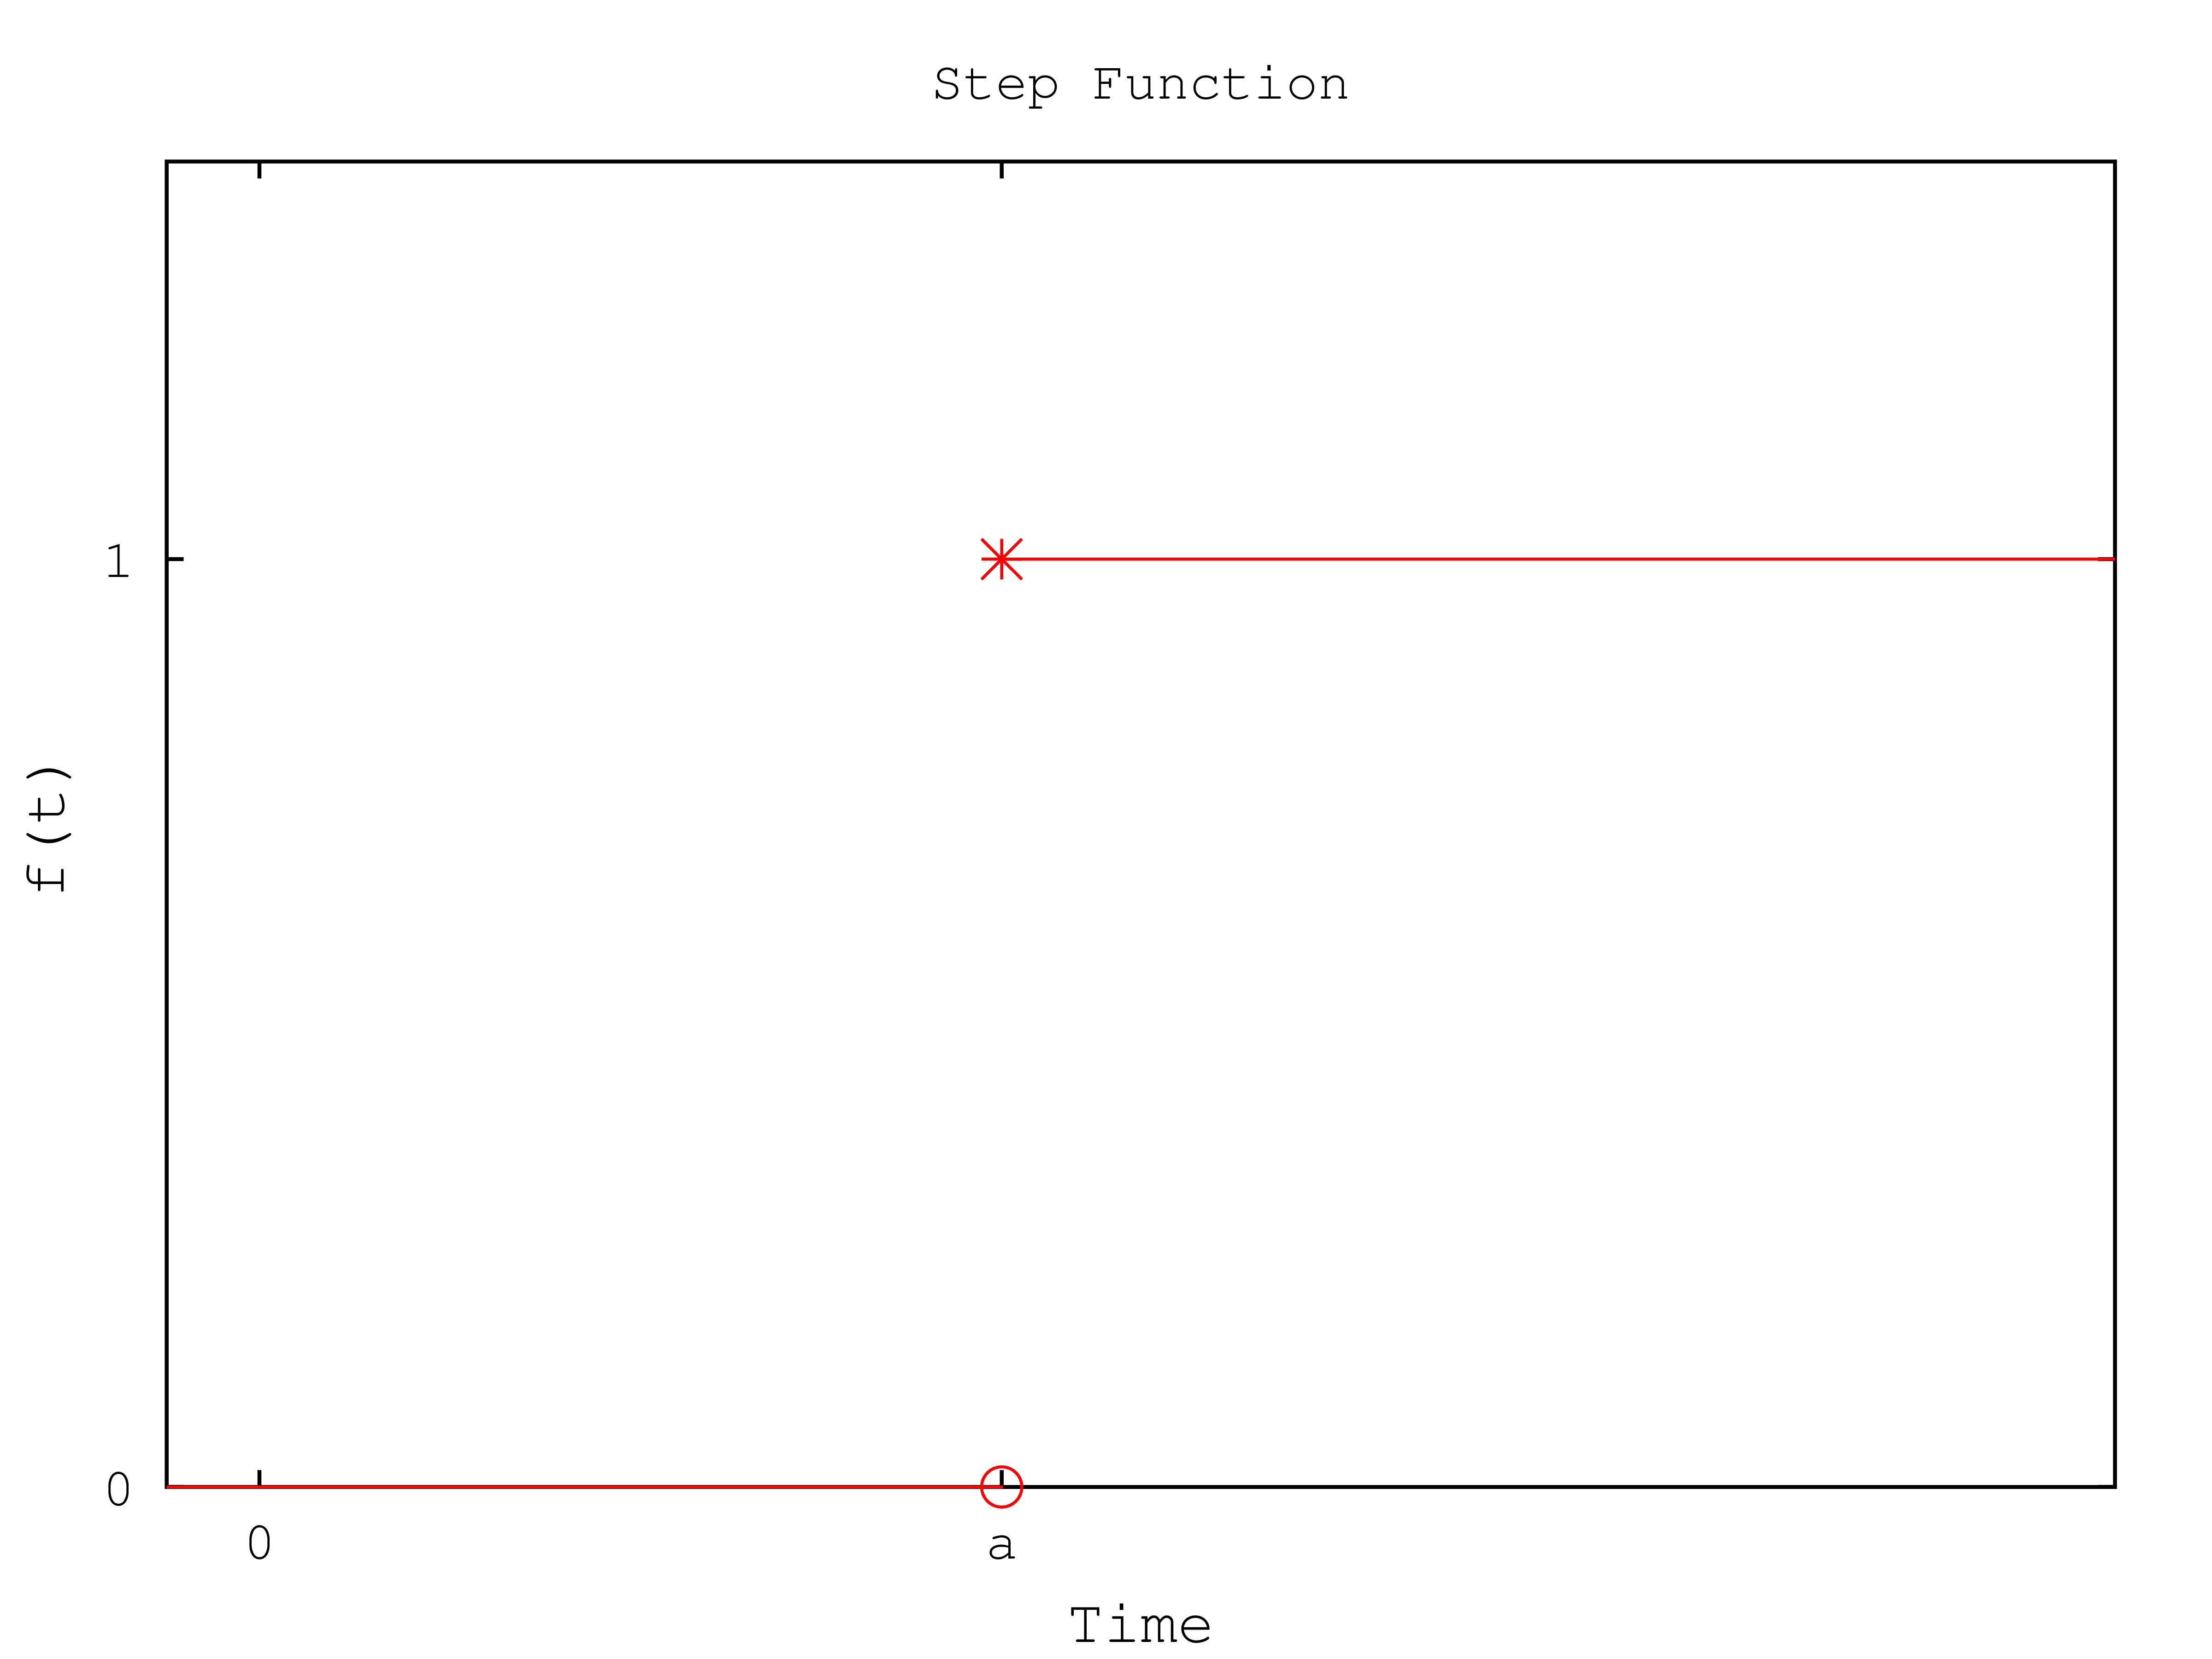
\includegraphics[width=5cm]{img/unitStepAta}}

  \uncover<2->
  {%

    Despite what you may have heard, nature is not continuous, and it
    is not differentiable.  In mechanican systems switches flip on and
    off, and things break. A function like this could be used to
    describe piecewise defined functions and help us deal with
    discontinuous functions. (We will see how later.)

  }

\end{frame}

\begin{frame}
  \frametitle{The Unit Step Function}

  \centerline{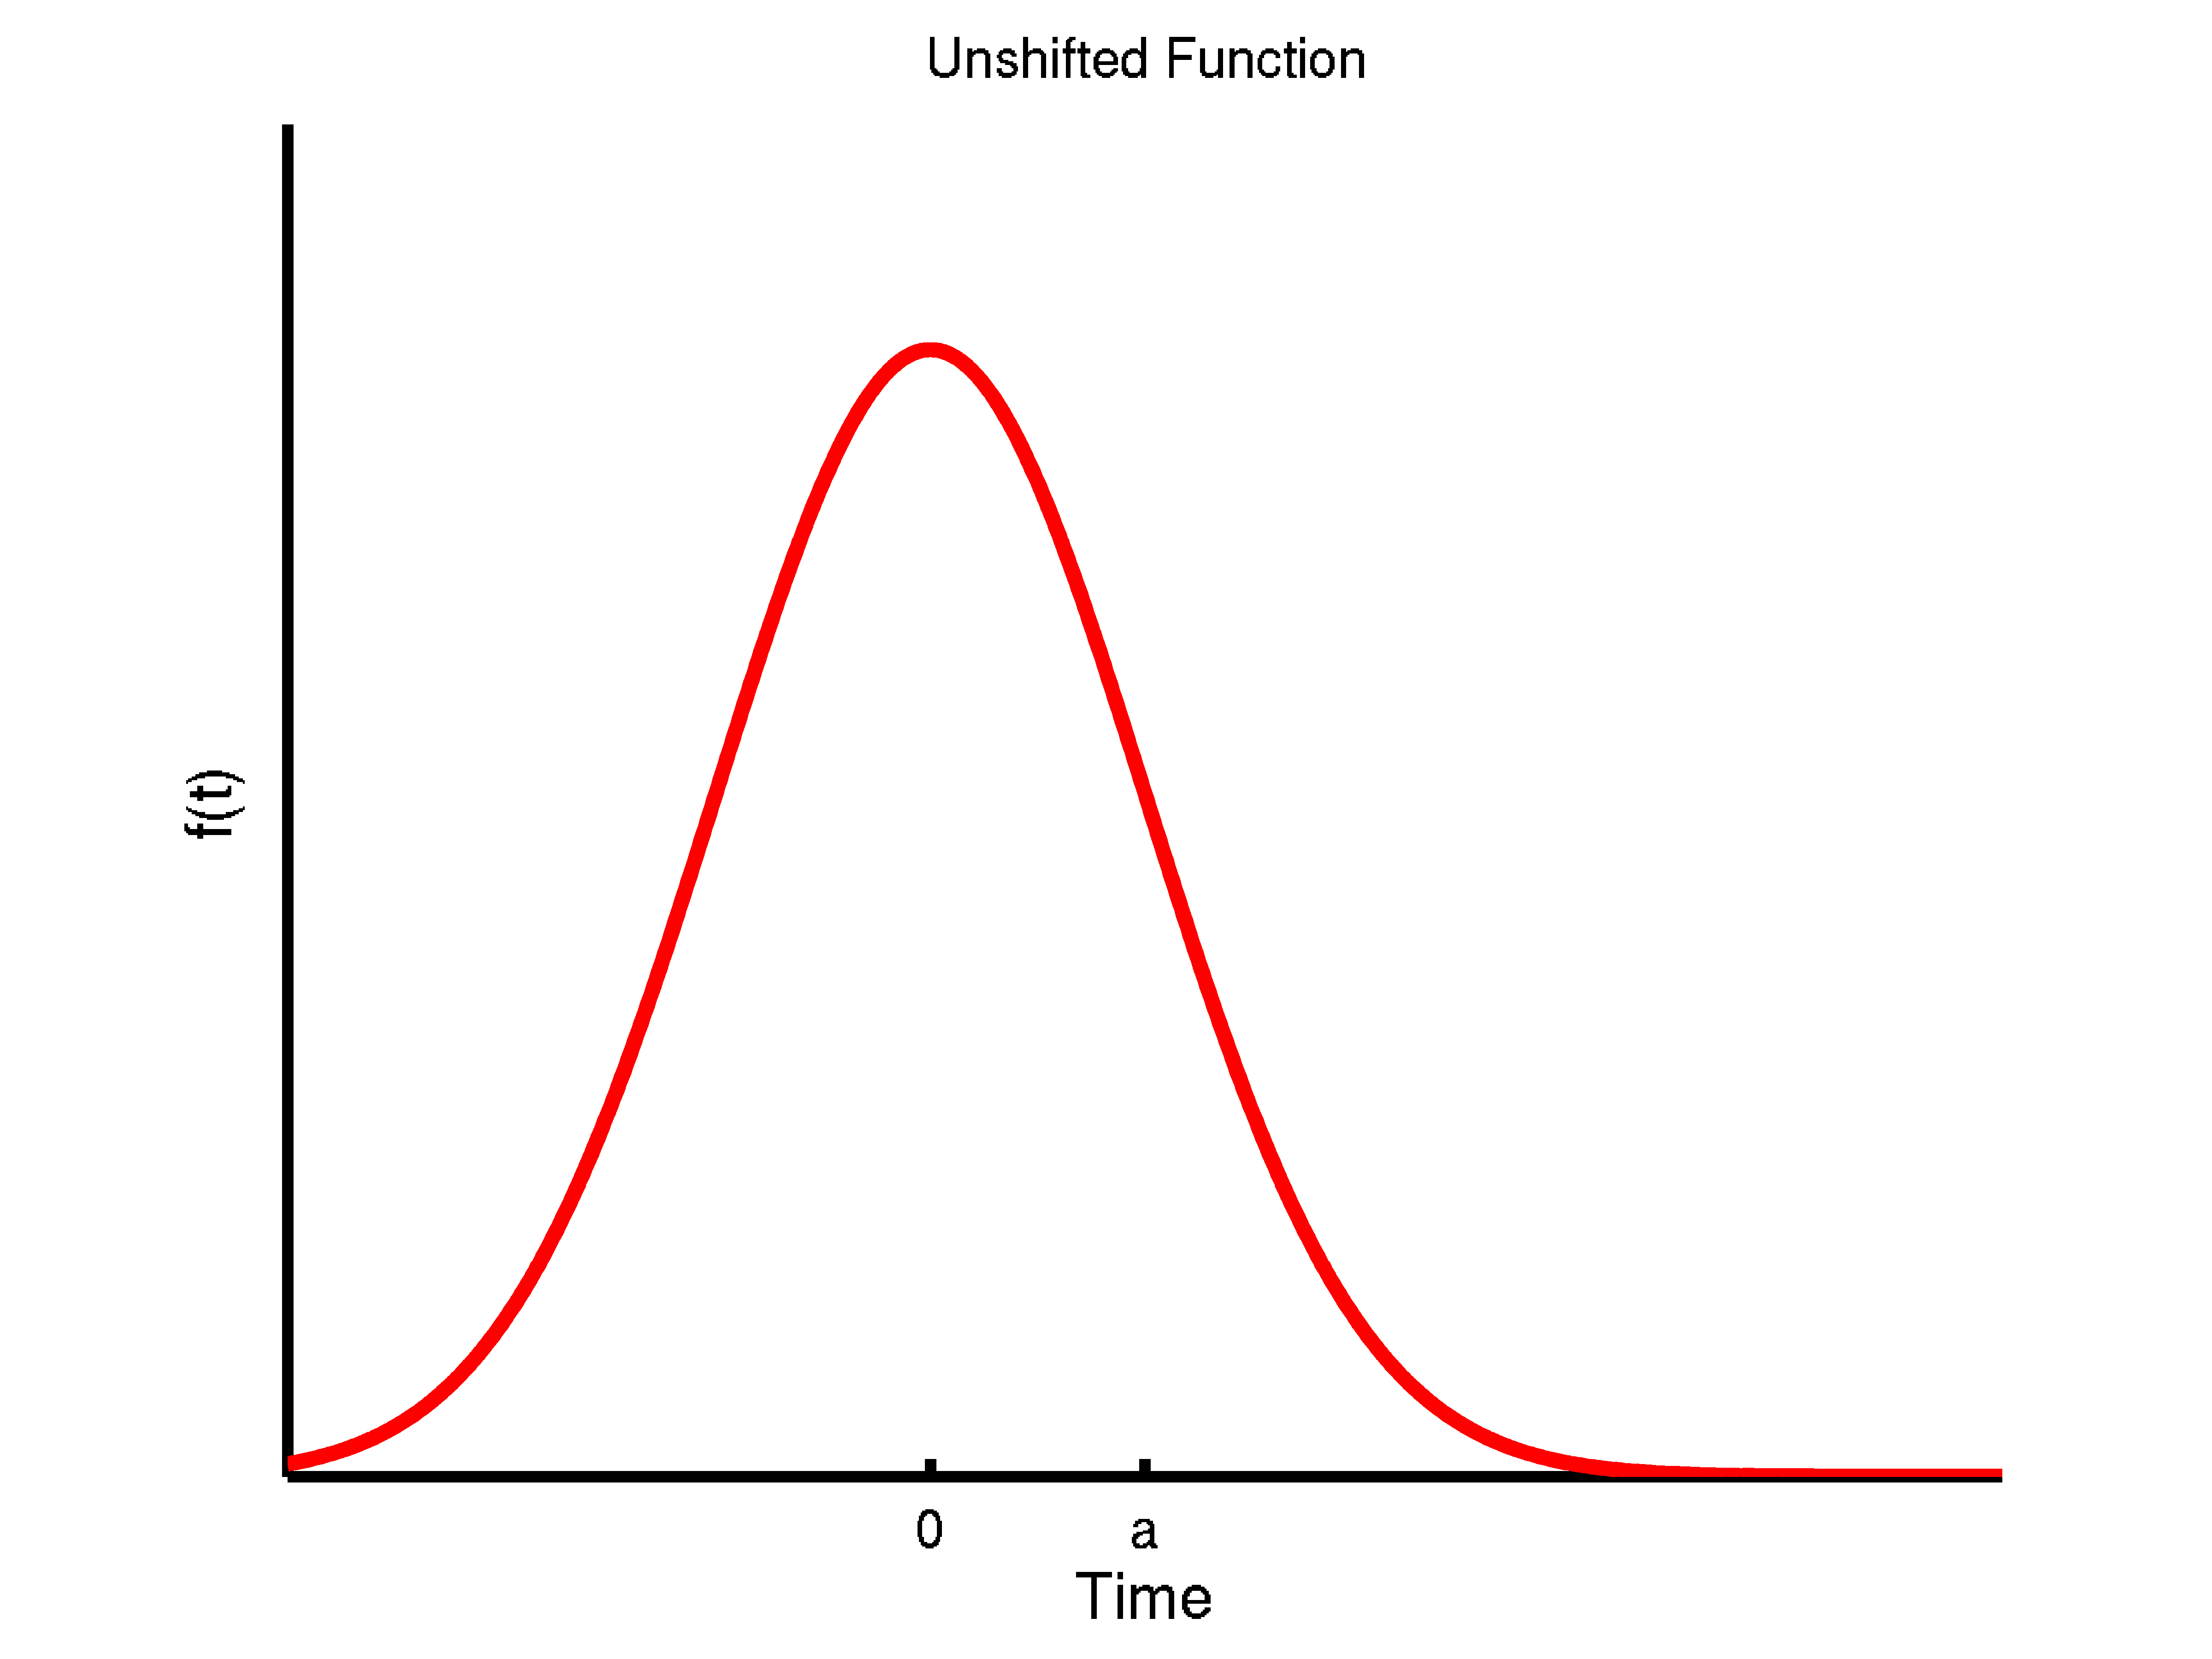
\includegraphics[width=5cm]{img/unshifted}}

  A new name for an old function:
  \begin{eqnarray*}
    f(t) & = & 
    \left\{
      \begin{array}{r@{\hspace{2em}}rcl}
        1 & t & \geq & 0 \\
        0 & t & < & 0
      \end{array}
    \right.
  \end{eqnarray*}

  \uncover<2->
  {
    Define this to be
    \begin{eqnarray*}
      \mathrm{step}(t) & = & 
      \left\{
        \begin{array}{r@{\hspace{2em}}rcl}
          1 & t & \geq & 0 \\
          0 & t & < & 0
        \end{array}
      \right.
    \end{eqnarray*}
  }

\end{frame}


\begin{frame}
  \frametitle{Shifted Version}

  \centerline{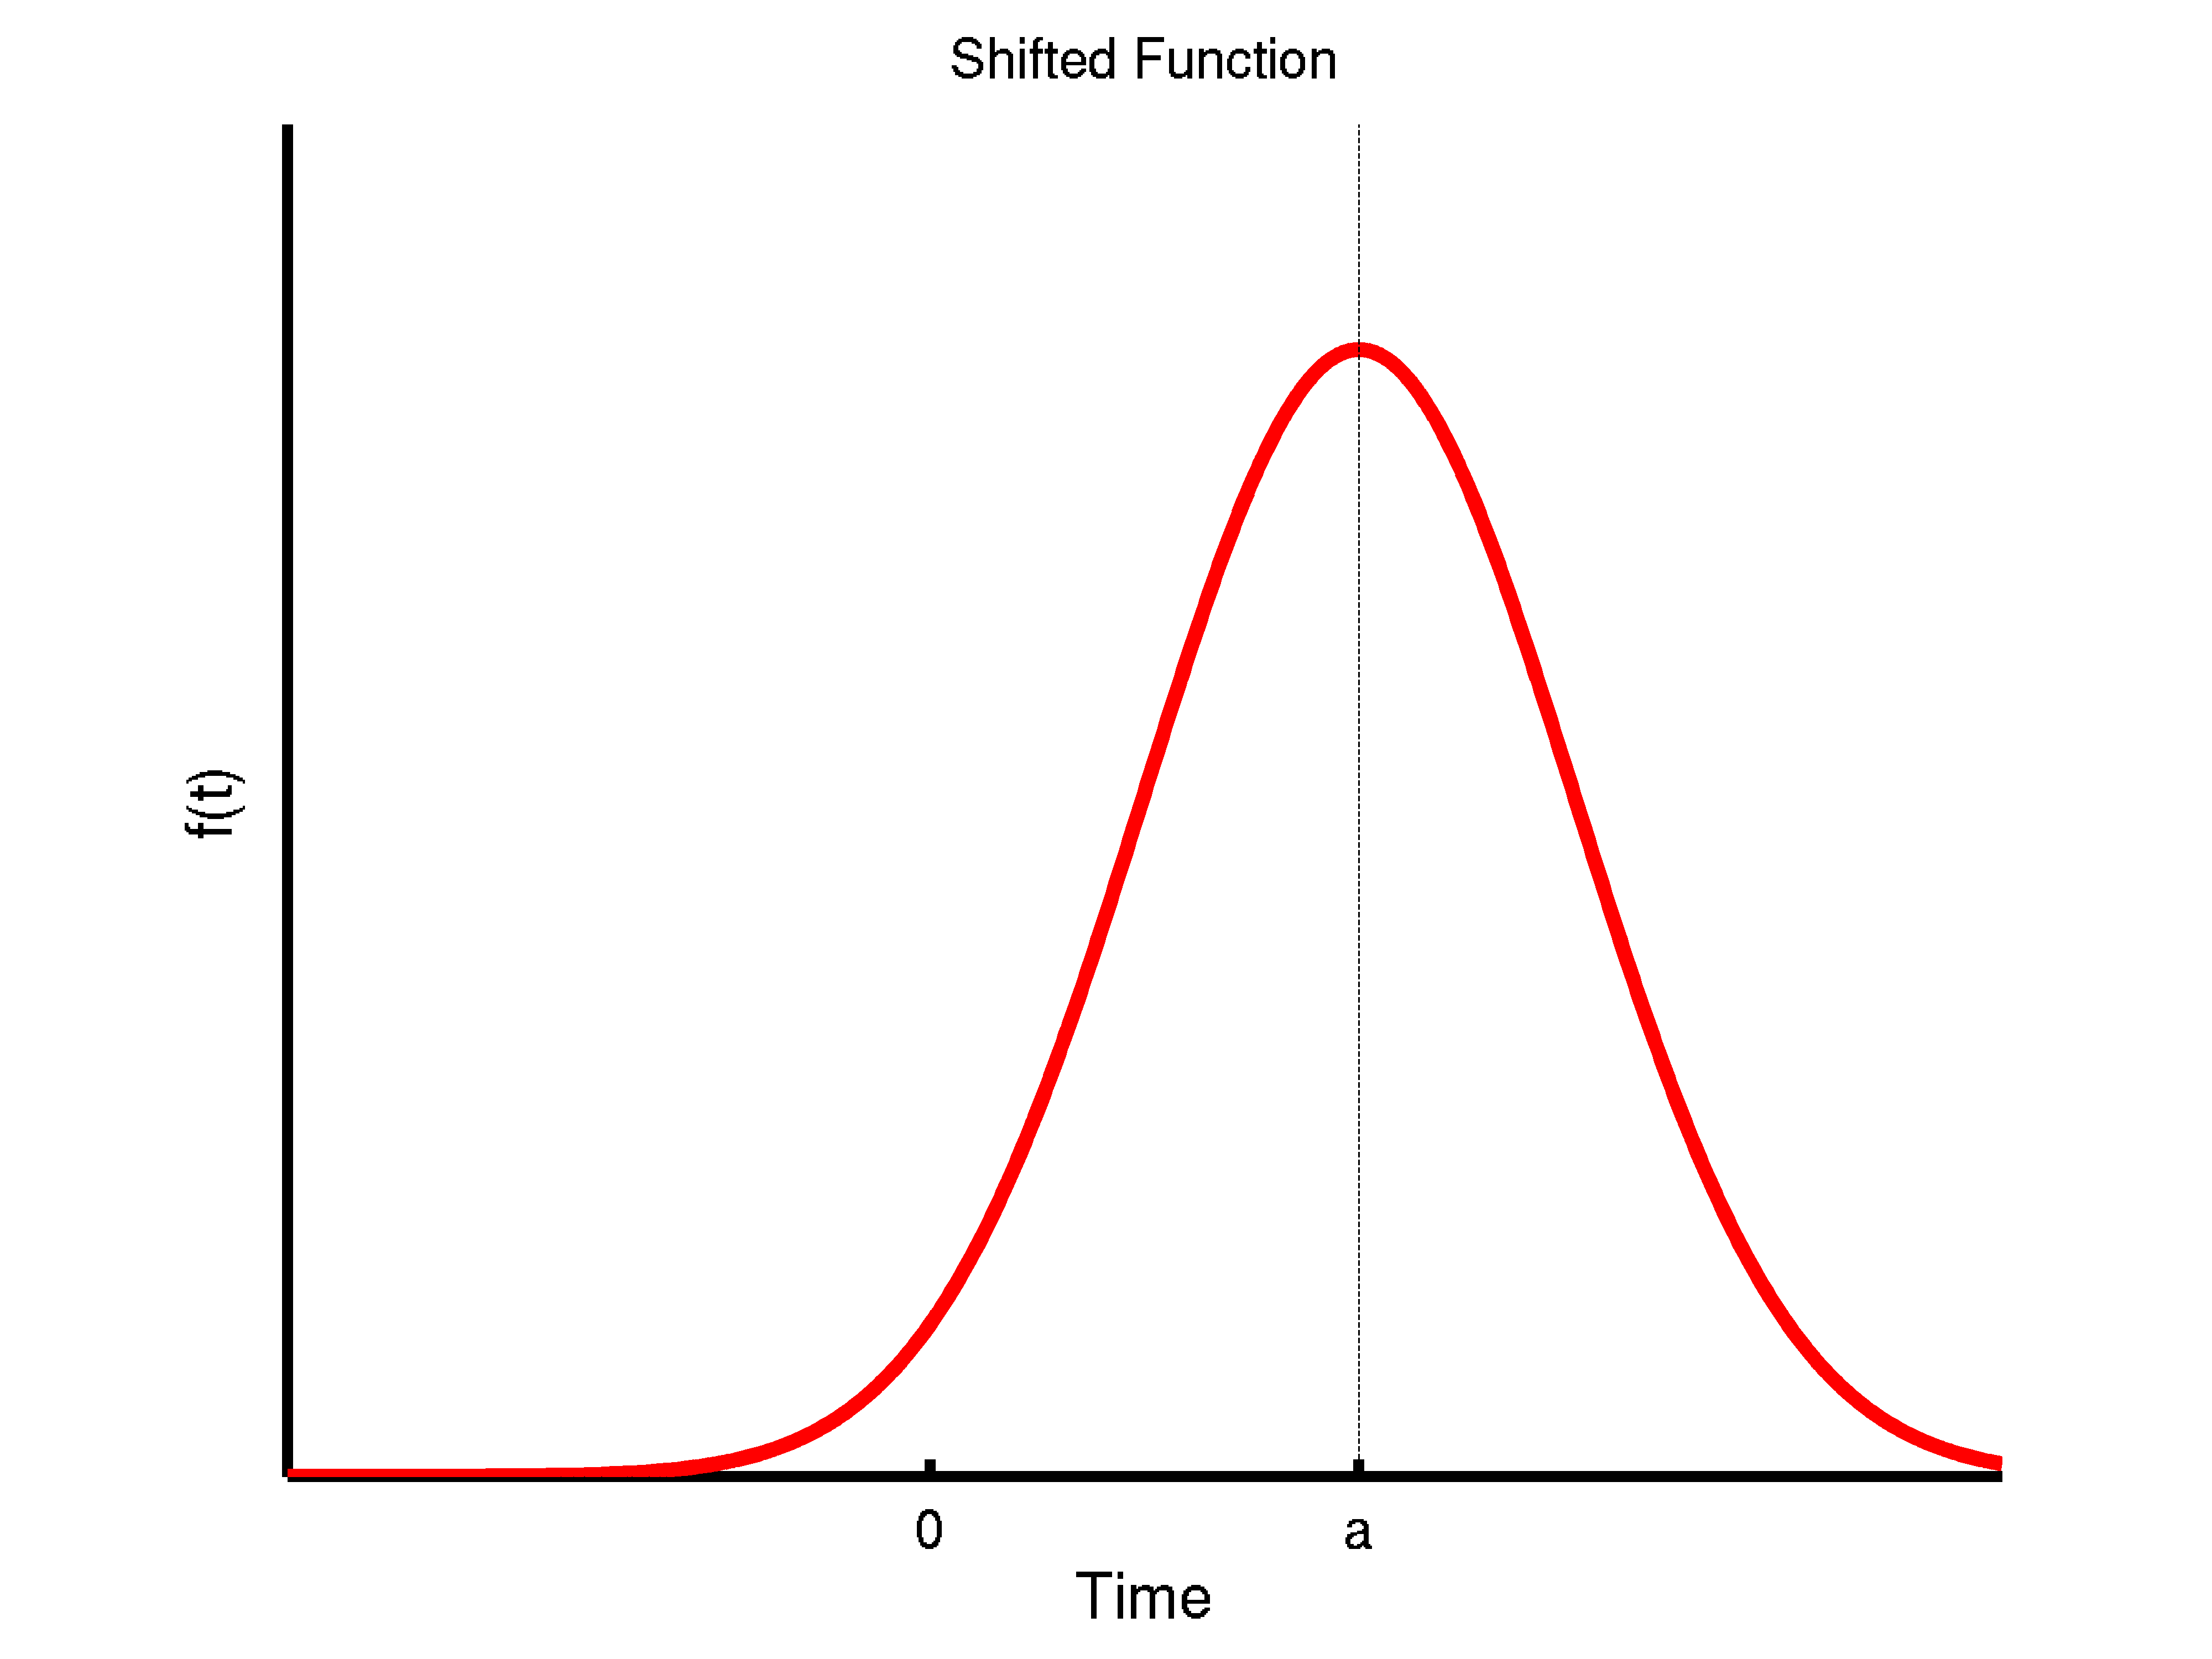
\includegraphics[width=5cm]{img/shifted}}

    The function shifted $a$ units to the right is
    \begin{eqnarray*}
      \mathrm{step}(t-a) & = & 
      \left\{
        \begin{array}{r@{\hspace{2em}}rcl}
          1 & t & \geq & a \\
          0 & t & < & a
        \end{array}
      \right.
    \end{eqnarray*}


\end{frame}

\subsection{Examples Using the Unit Step Function}

\begin{frame}
  \frametitle{So What?}

  \centerline{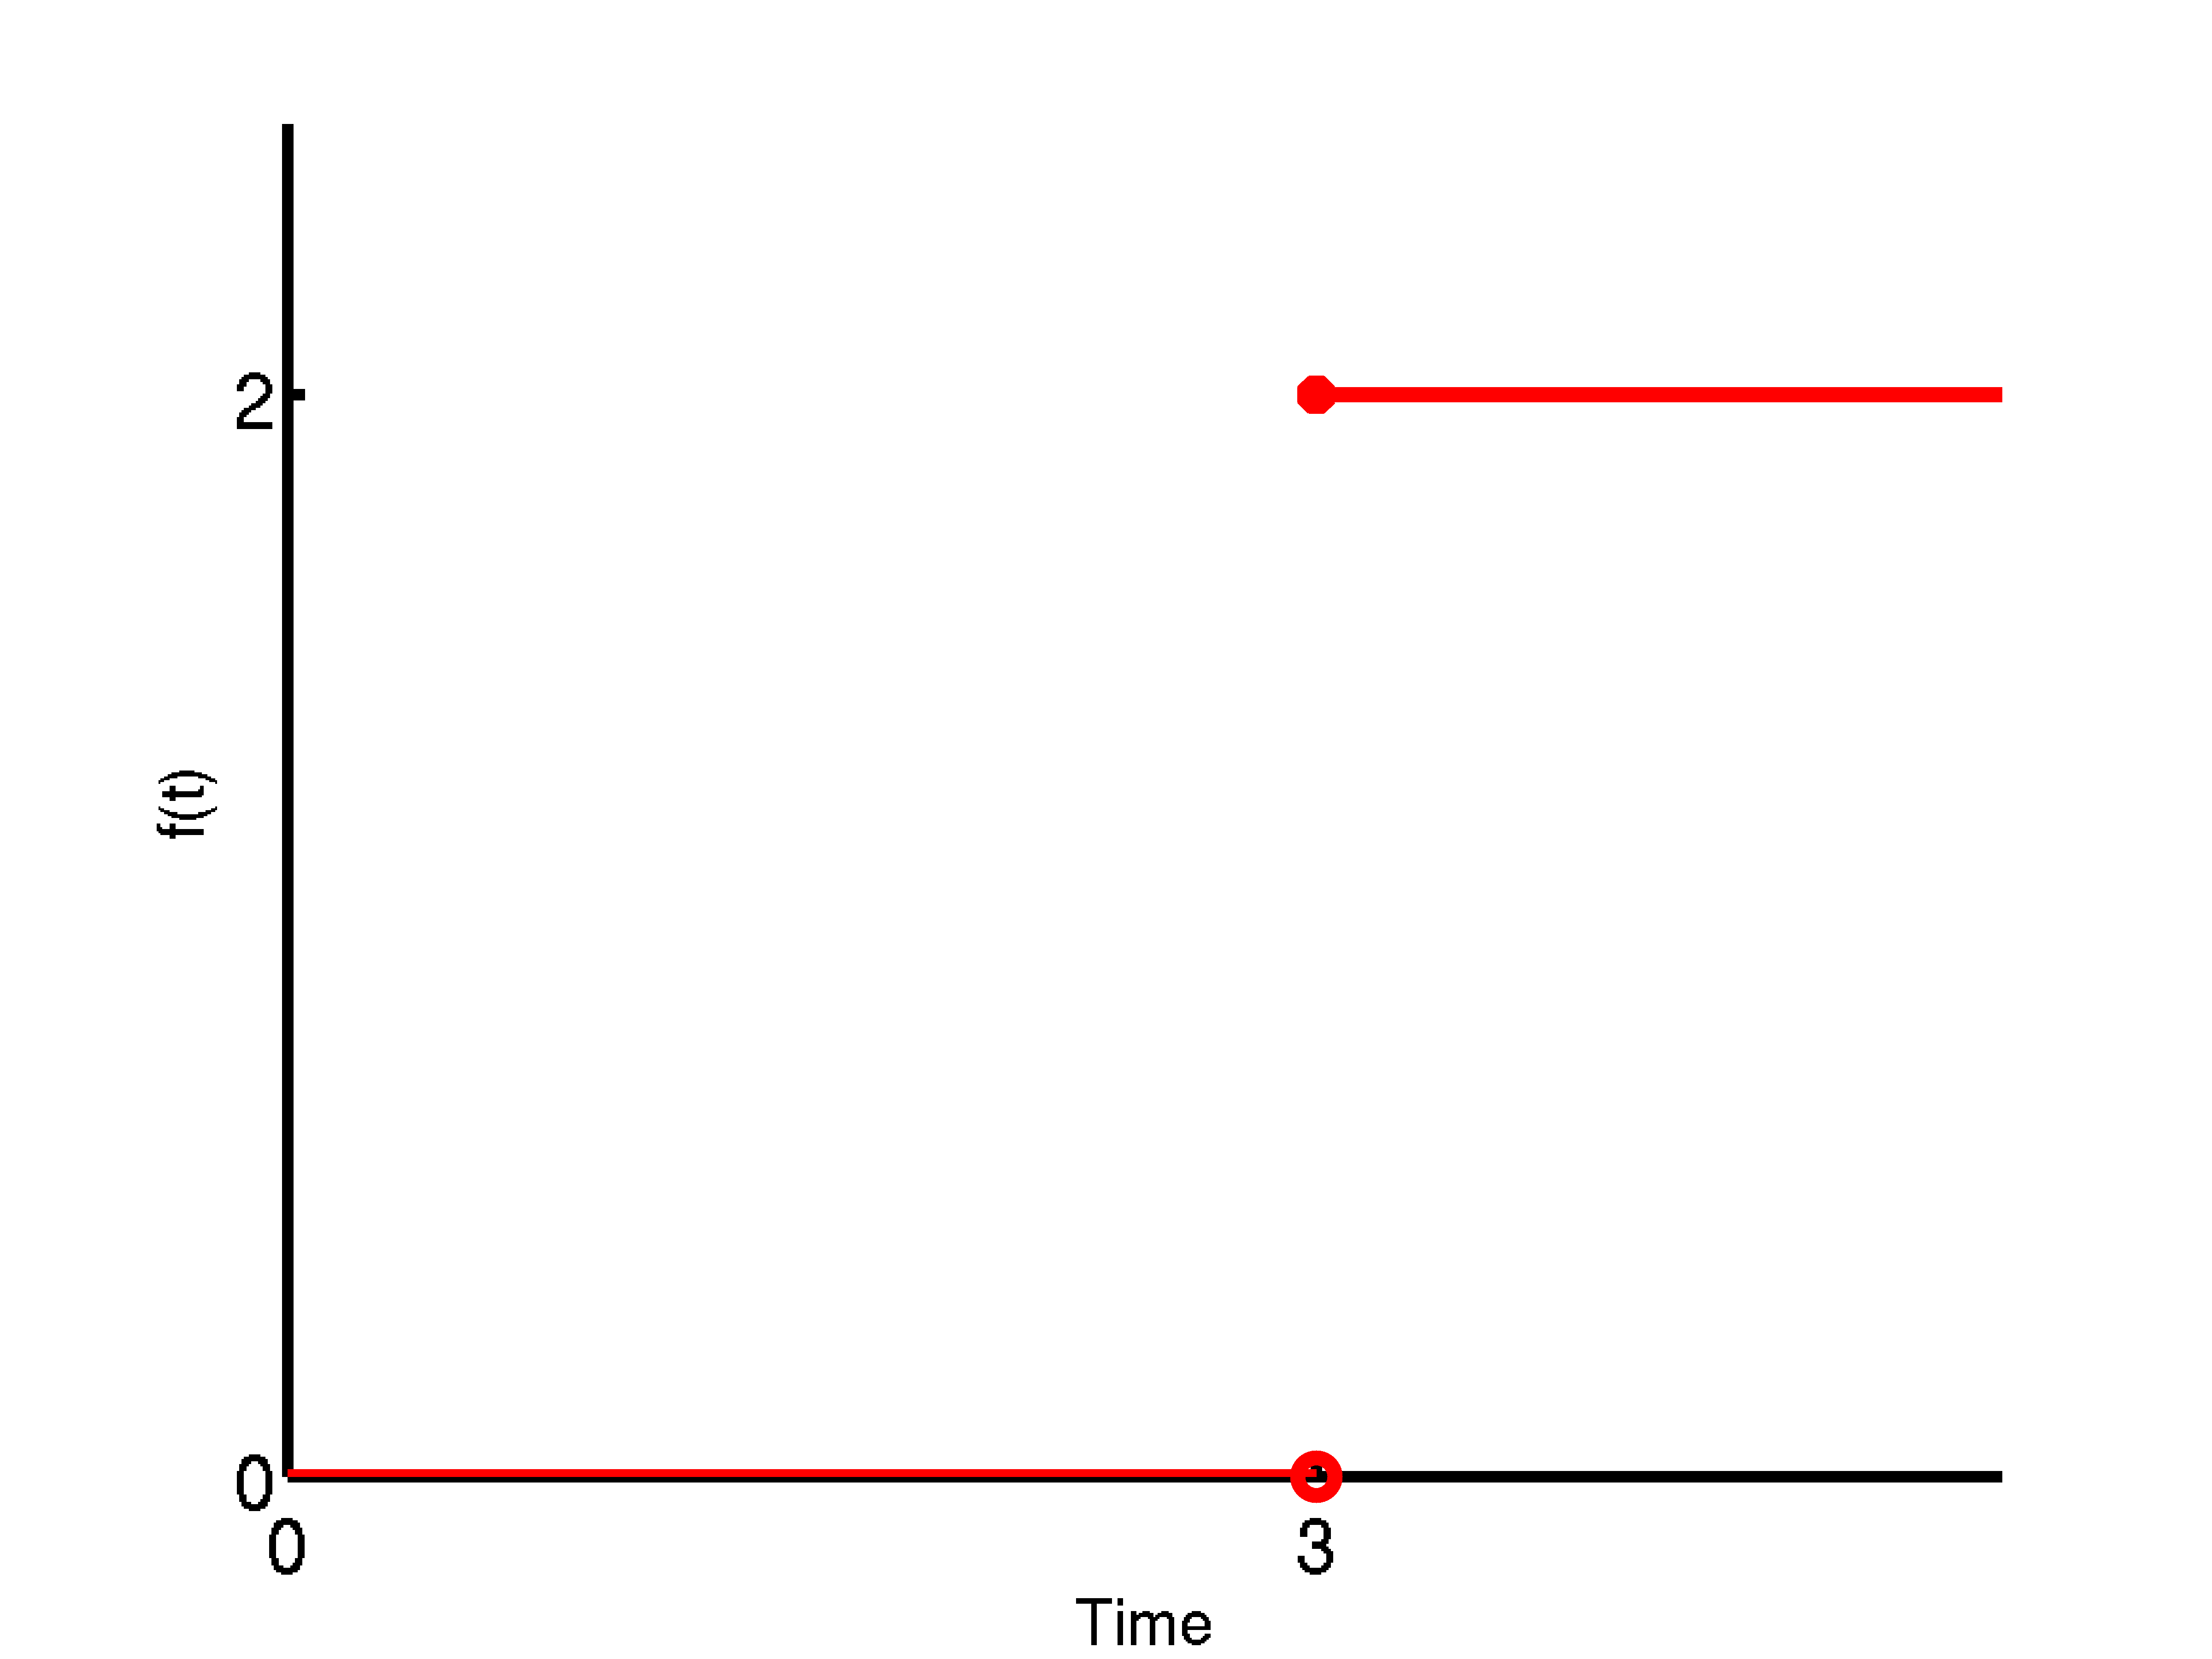
\includegraphics[width=5cm]{img/stepEx1}}

  \begin{eqnarray*}
      f(t) & = & 
      \left\{
        \begin{array}{r@{\hspace{2em}}rcl}
          2 & t & \geq & 3 \\
          0 & t & < & 3
        \end{array}
      \right.
  \end{eqnarray*}

  \uncover<2->
  {
    \begin{eqnarray*}
      f(t) & = & 2\mathrm{step}(t-3).
    \end{eqnarray*}
  }

\end{frame}


\begin{frame}
  \frametitle{A little bit harder now}

  \centerline{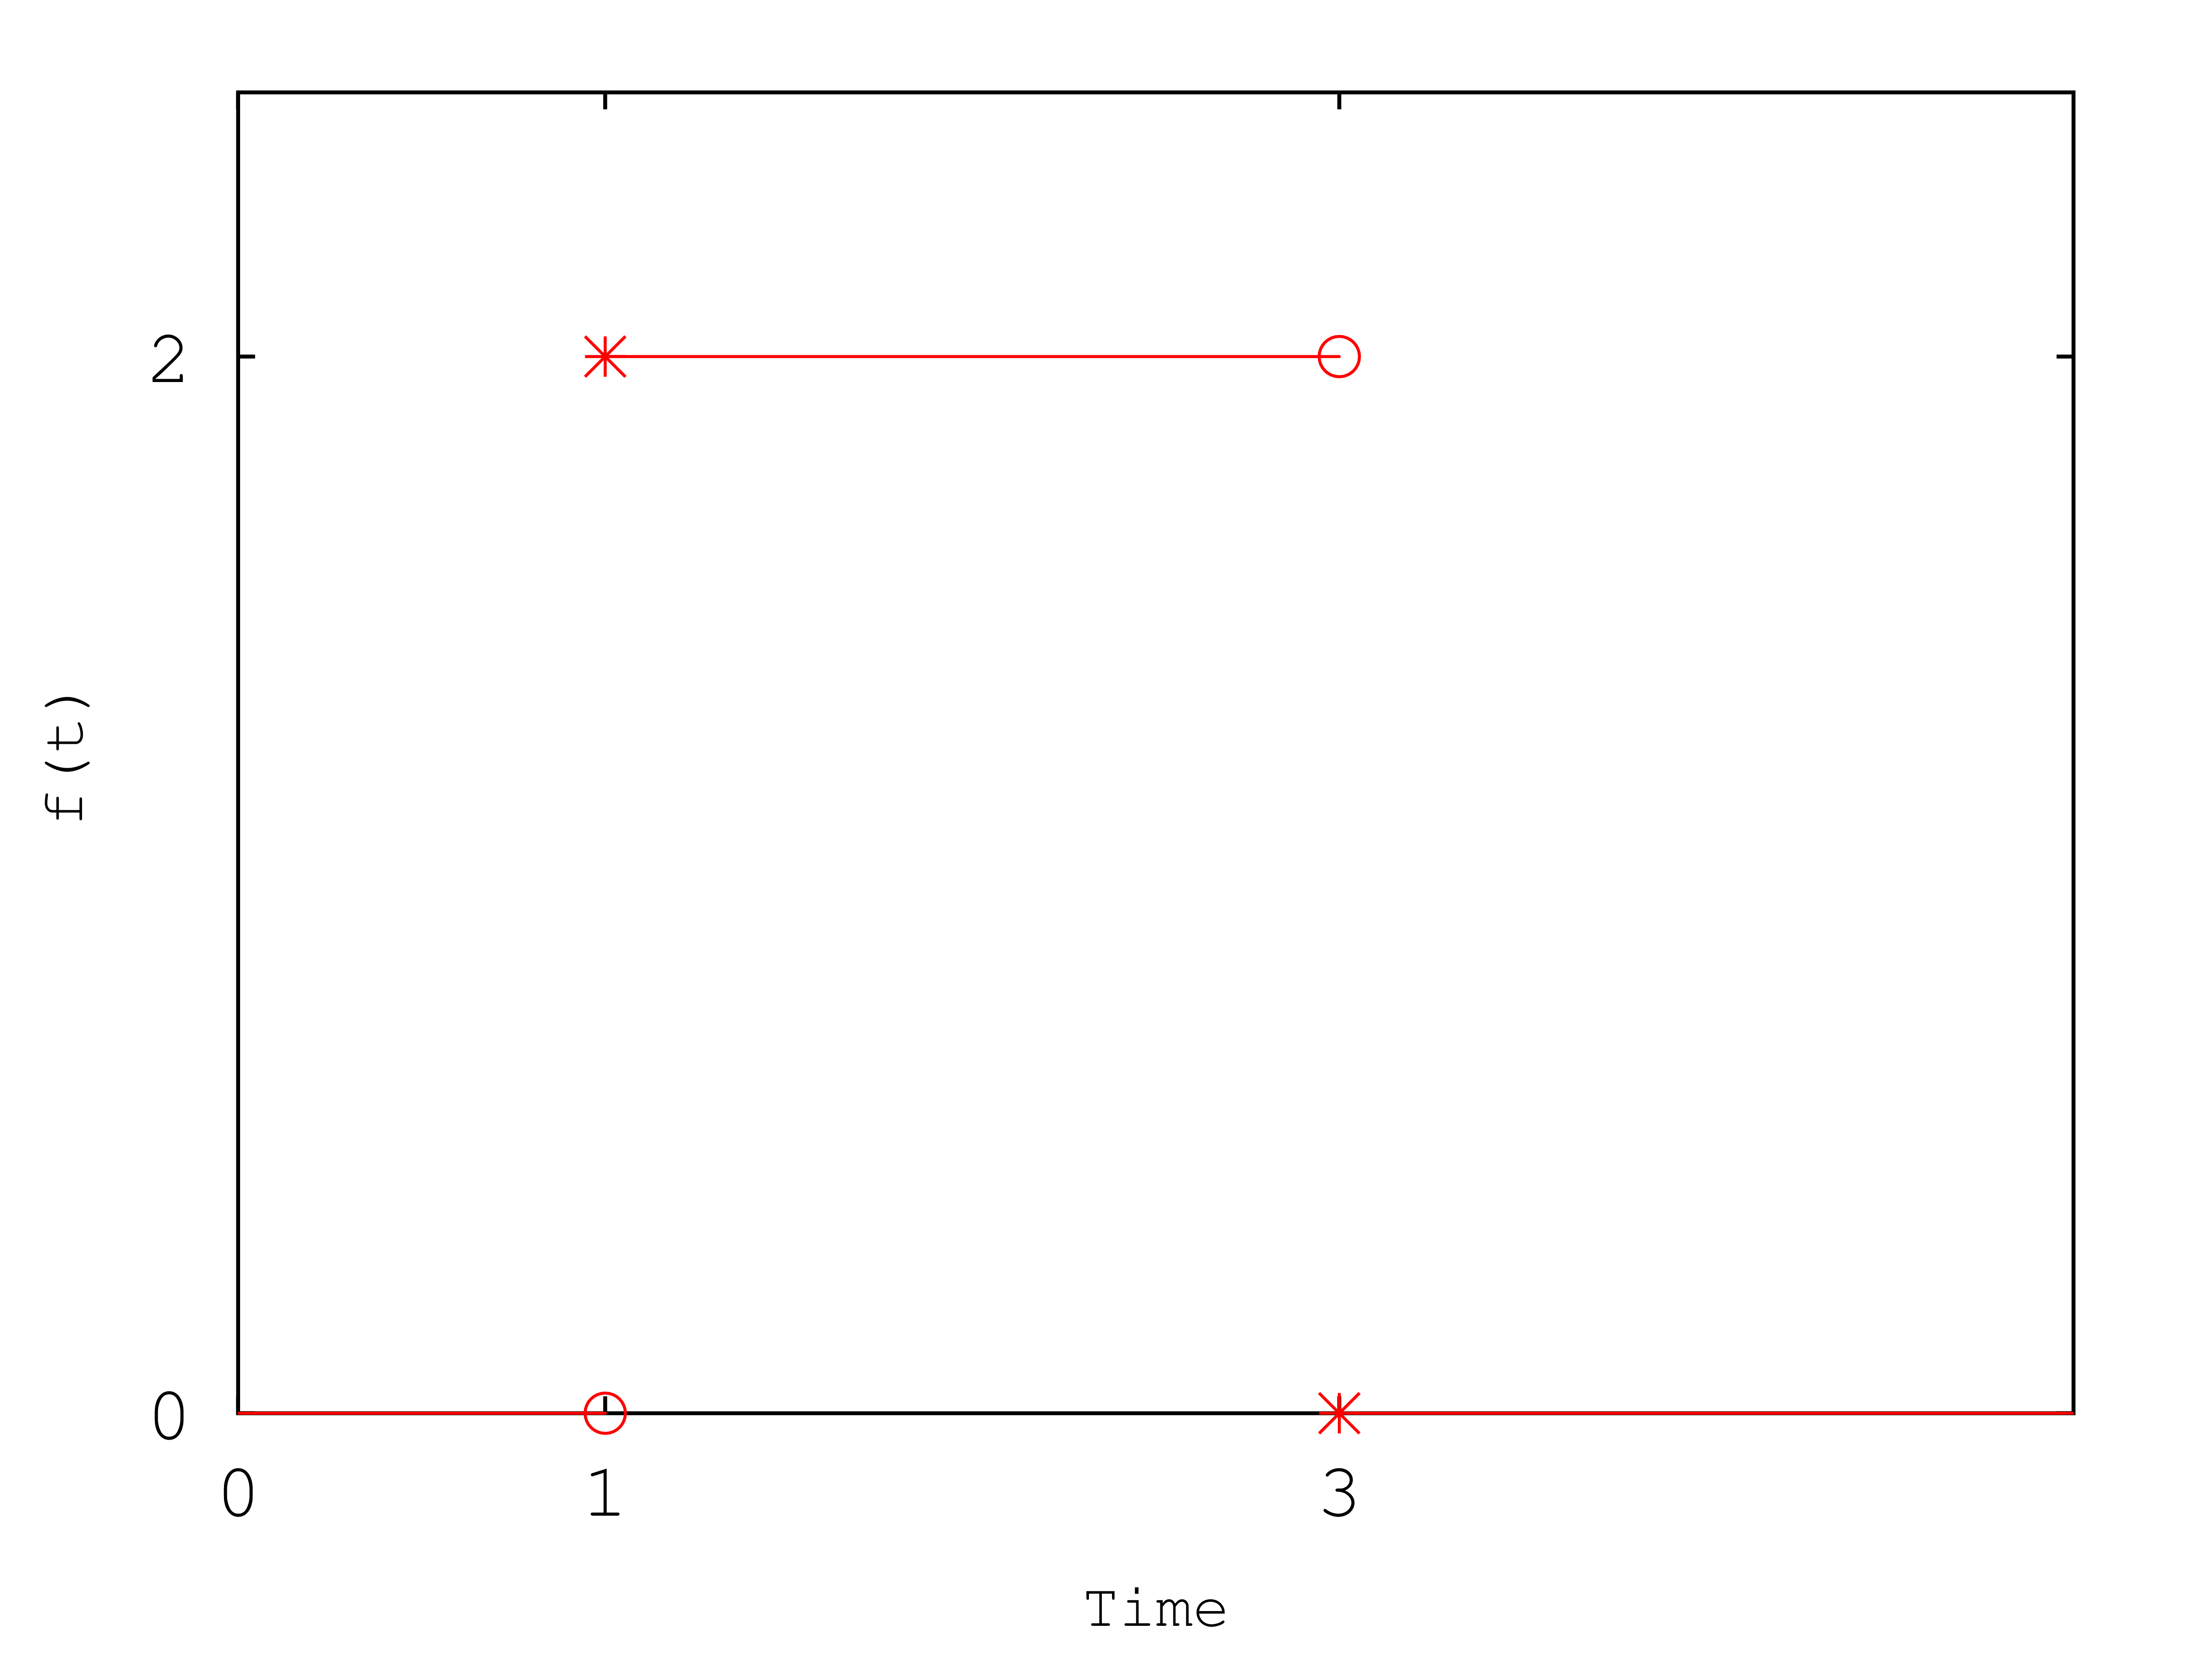
\includegraphics[width=5cm]{img/stepEx2}}

  \begin{eqnarray*}
      f(t) & = & 
      \left\{
        \begin{array}{rr}
          2 & 1\leq t < 3 \\
          0 & \mathrm{otherwise}
        \end{array}
      \right.
  \end{eqnarray*}

  \uncover<2->
  {
    \begin{eqnarray*}
      f(t) & = & 2\cdot\mathrm{step}(t-1) - 2\cdot\mathrm{step}(t-3).
    \end{eqnarray*}
  }

\end{frame}

\begin{frame}
  \frametitle{A little bit harder now}

  \centerline{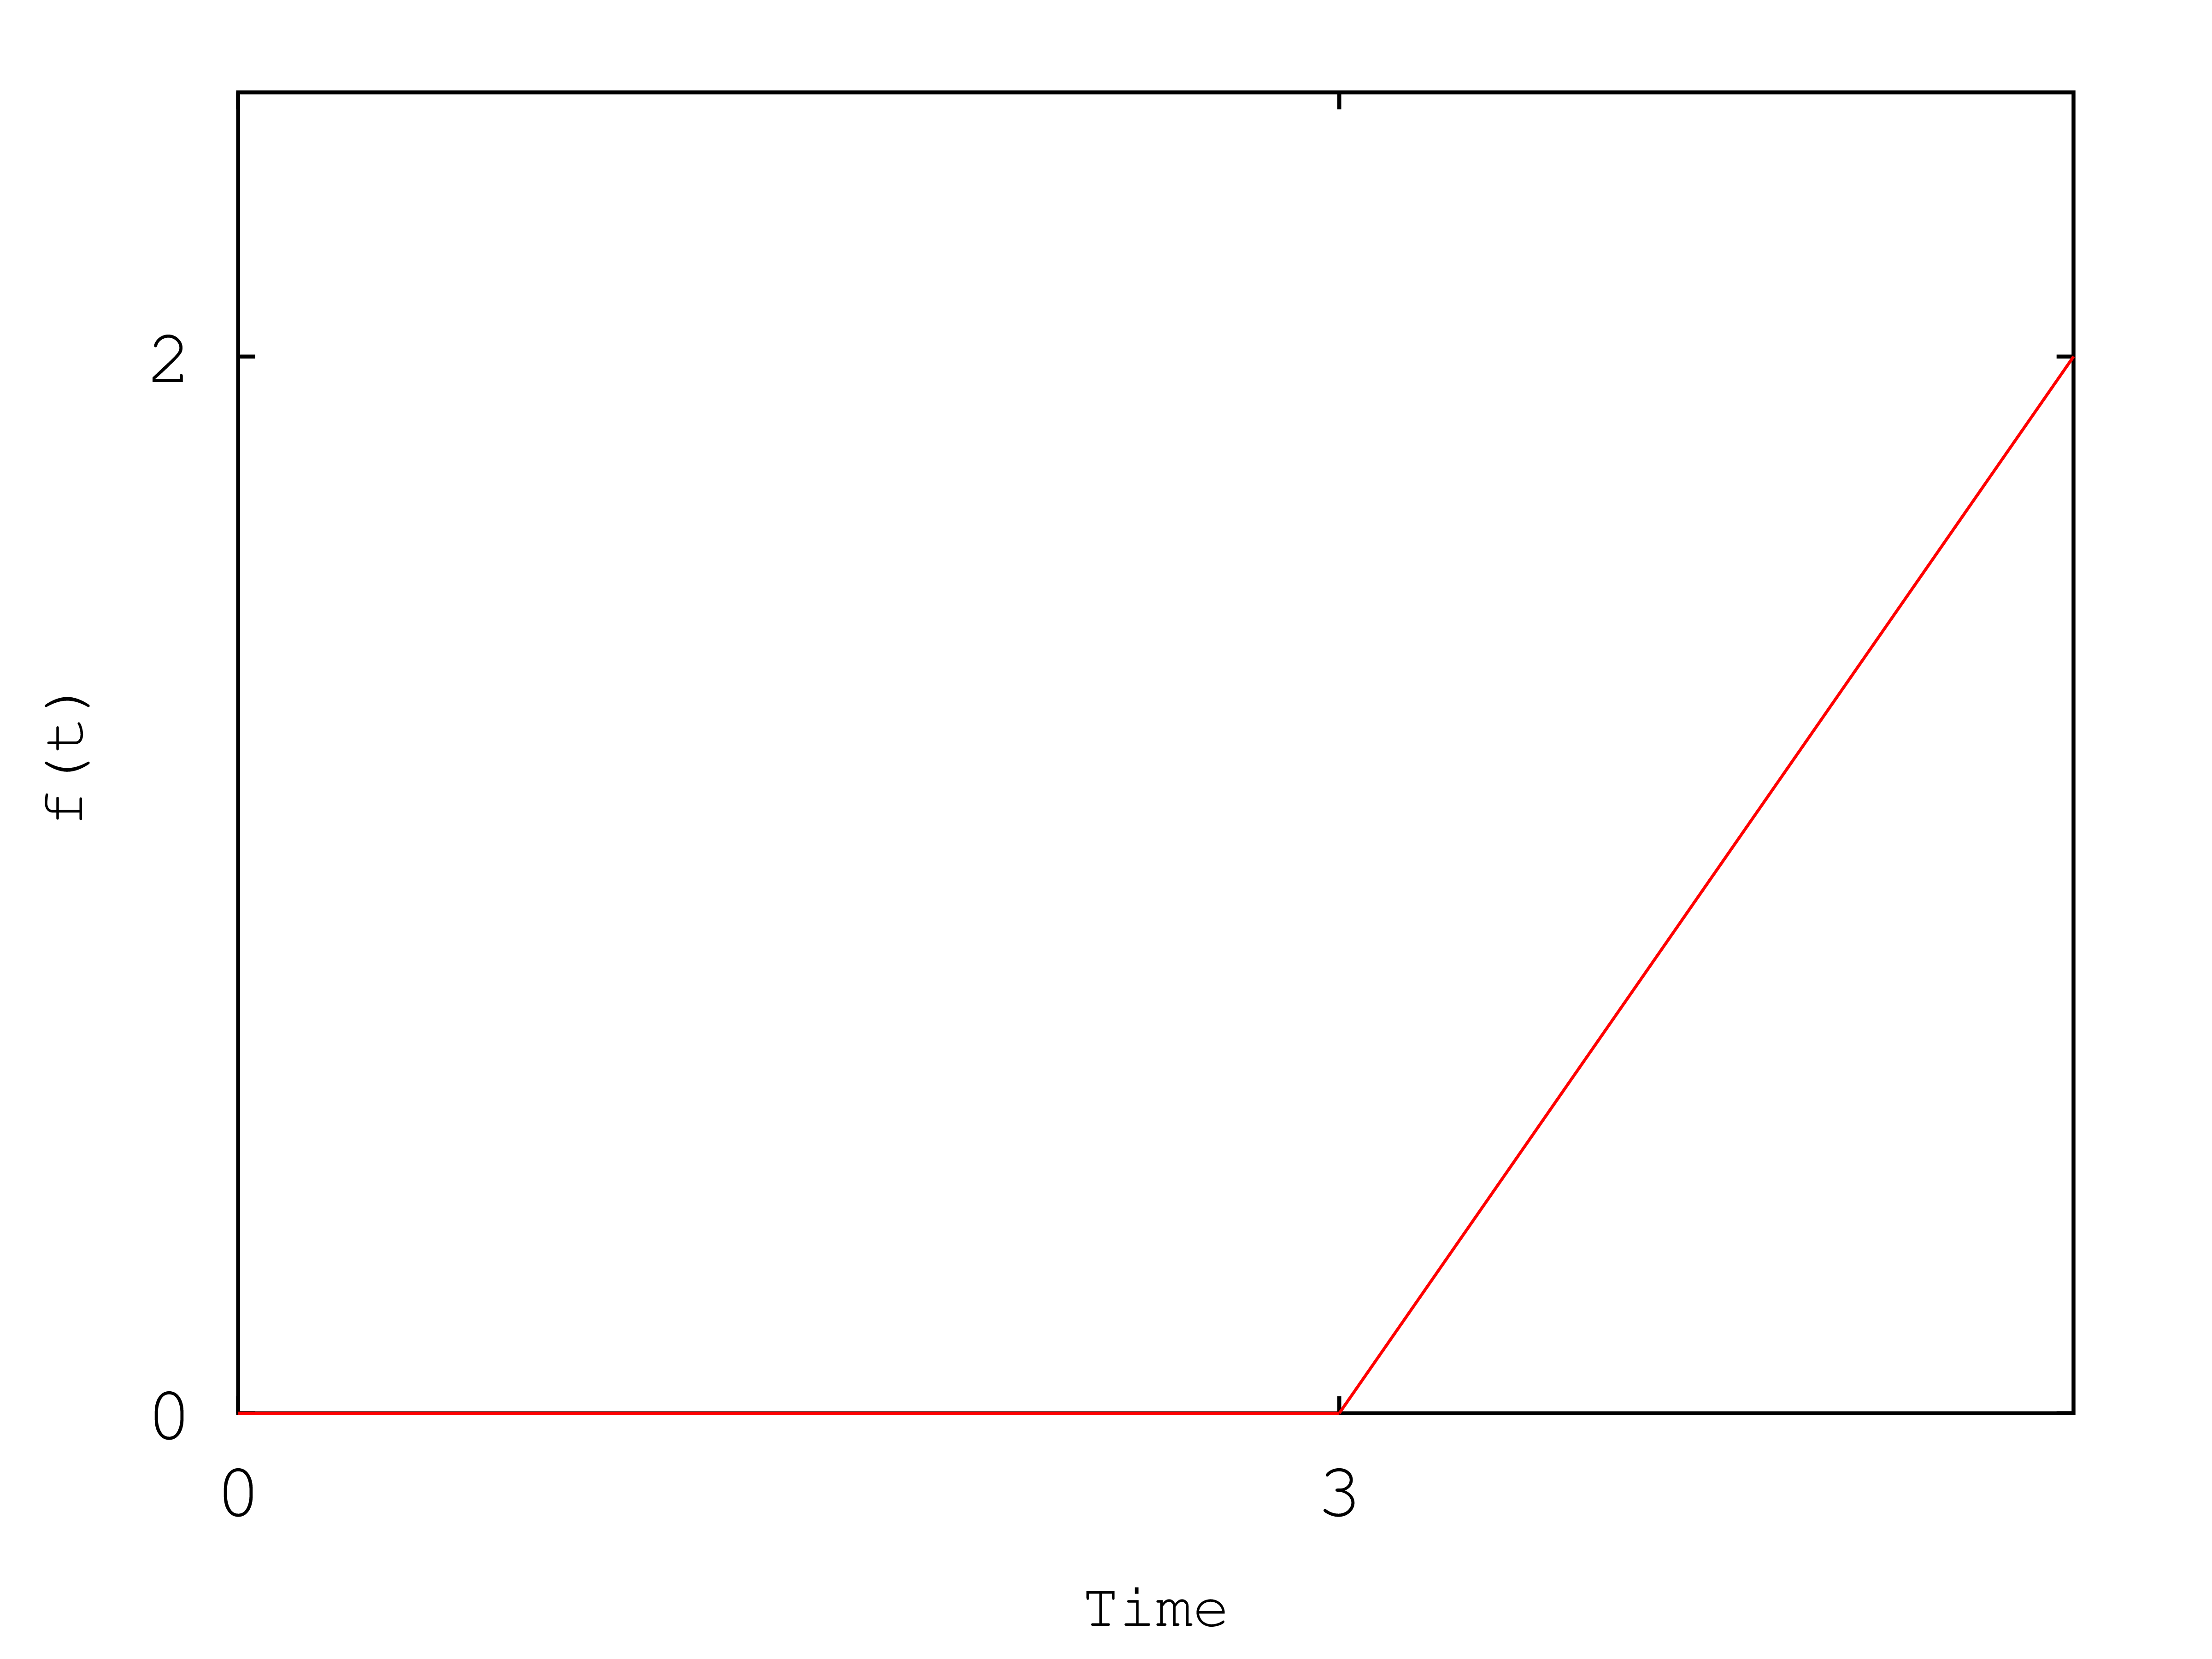
\includegraphics[width=5cm]{img/stepEx3}}

  \begin{eqnarray*}
      f(t) & = & 
      \left\{
        \begin{array}{rr}
          t-2 & 1\leq t < 3 \\
          0 & \mathrm{otherwise}
        \end{array}
      \right.
  \end{eqnarray*}

  \uncover<2->
  {
    \begin{eqnarray*}
      f(t) & = & (t-2)\cdot\mathrm{step}(t-1) - (t-2)\cdot\mathrm{step}(t-3).
    \end{eqnarray*}
  }

\end{frame}

\begin{frame}
  \frametitle{A little bit harder now}

  \centerline{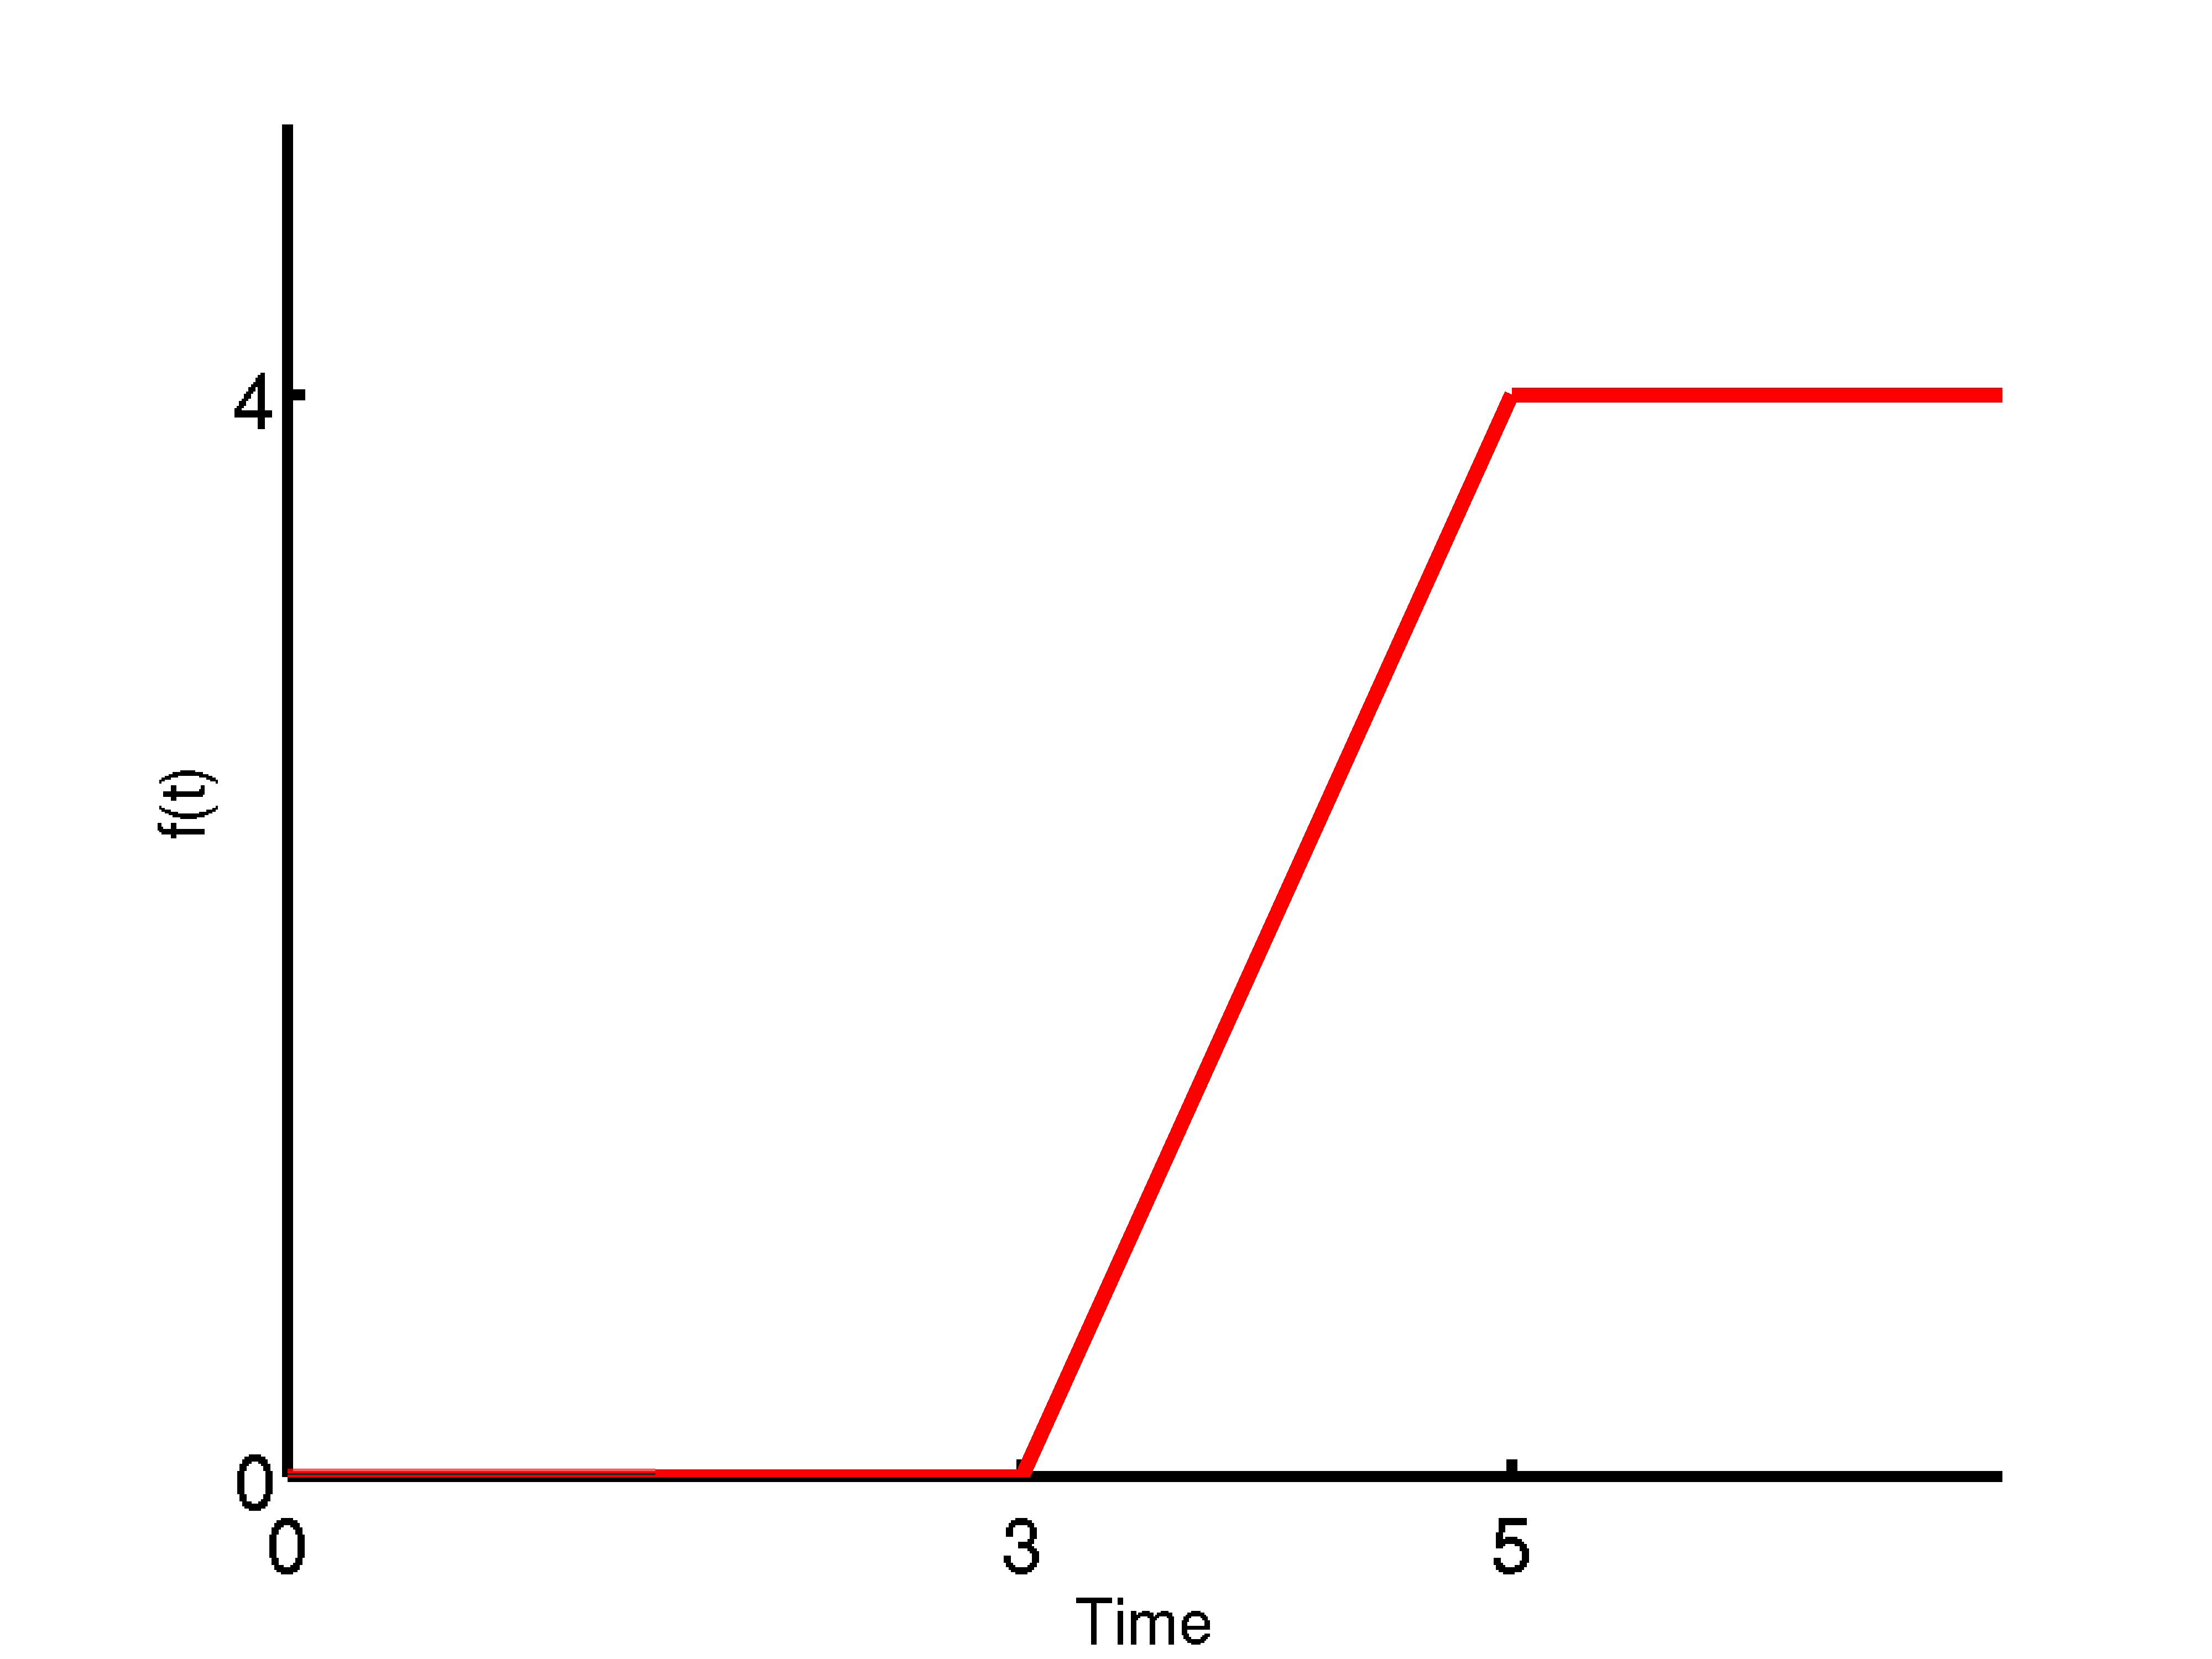
\includegraphics[width=5cm]{img/stepEx4}}

  \begin{eqnarray*}
      f(t) & = & 
      \left\{
        \begin{array}{r@{\hspace{2em}}rcccl}
          4 & t & \geq & 5 \\
          2(t-3) & 3 & < & t & < & 5 \\
          0 & t & \leq 3 
        \end{array}
      \right.
  \end{eqnarray*}

  \uncover<2->
  {
    \begin{eqnarray*}
      f(t) & = & 2(t-3)\cdot\mathrm{step}(t-3) -
      2(t-3)\cdot\mathrm{step}(t-5) + 4\cdot\mathrm{step}(t-5).
    \end{eqnarray*}
  }


\end{frame}


\begin{frame}
  \frametitle{A little bit harder now}

  \centerline{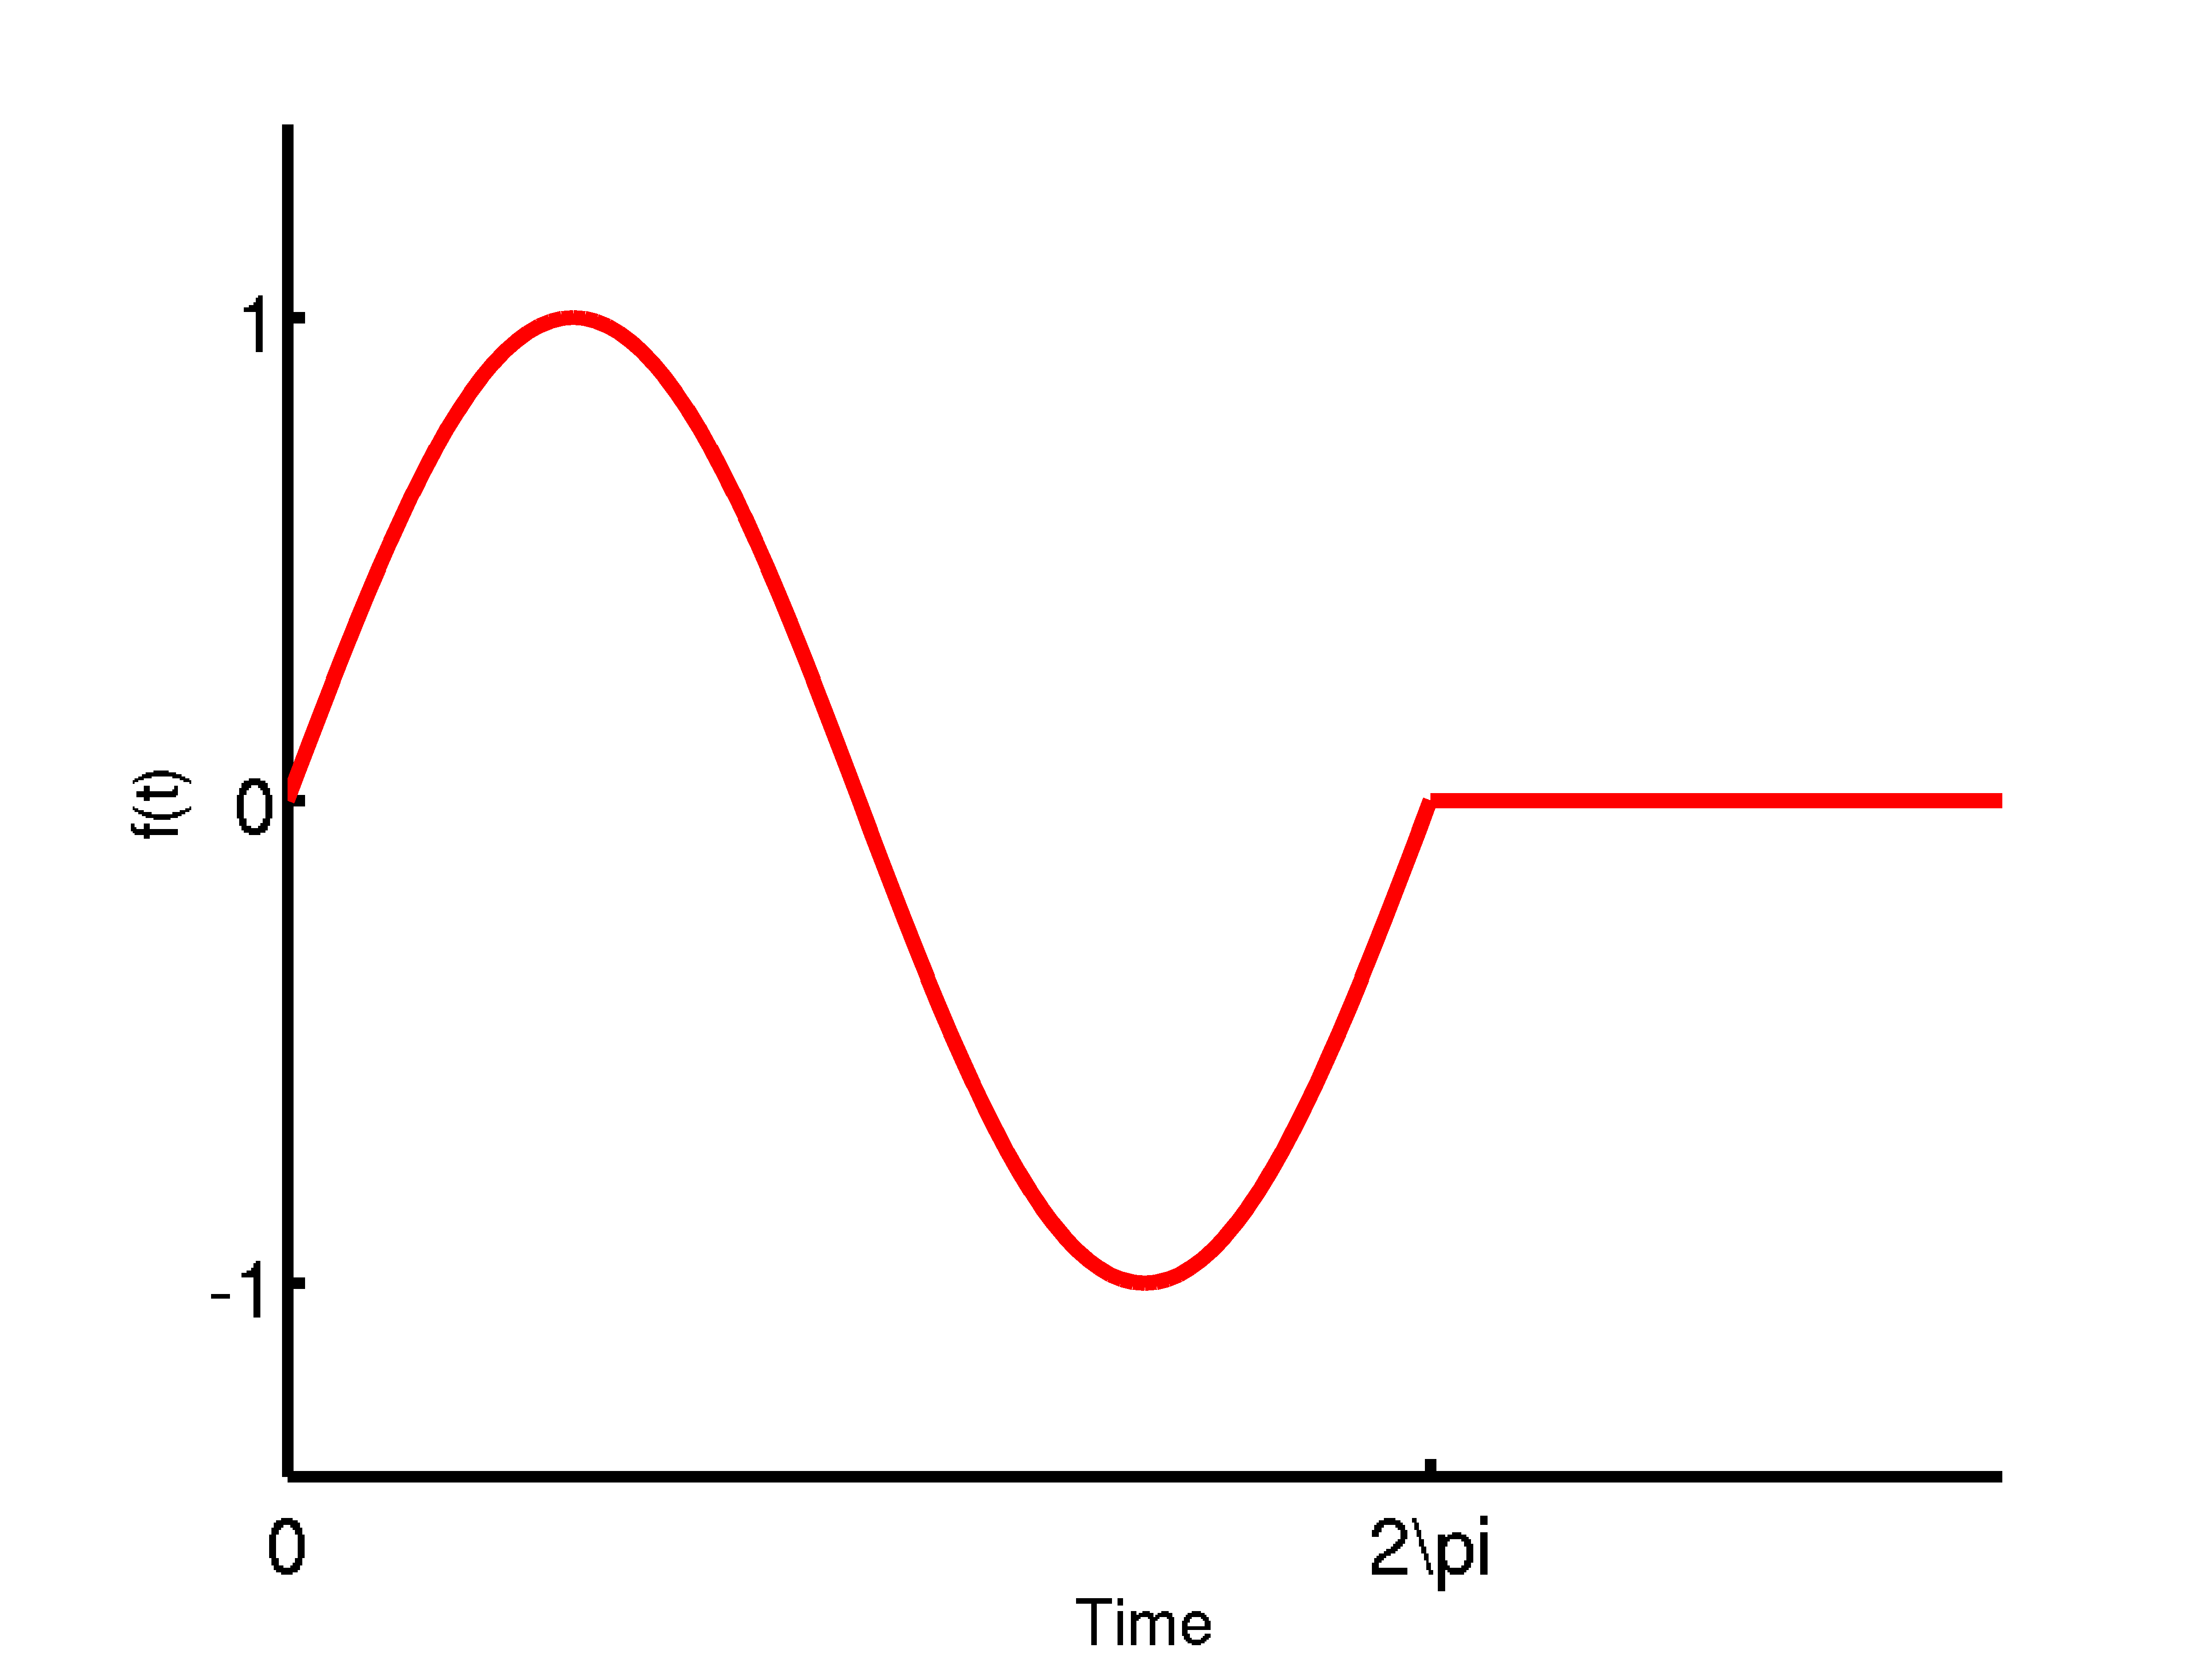
\includegraphics[width=5cm]{img/stepEx5}}

  \begin{eqnarray*}
      f(t) & = & 
      \left\{
        \begin{array}{r@{\hspace{2em}}r}
          \sin(t) & 0 \leq t \leq 2\pi \\
          0 &  \mathrm{otherwise}.
        \end{array}
      \right.
  \end{eqnarray*}

  \uncover<2->
  {
    \begin{eqnarray*}
      f(t) & = & \sin(t)\mathrm{step}(t-0) - \sin(t)\mathrm{step}(t-2\pi).
    \end{eqnarray*}
  }


  \uncover<3->
  {
    Assume that $t\geq 0$:
    \begin{eqnarray*}
      f(t) & = & \sin(t) - \sin(t)\mathrm{step}(t-2\pi).
    \end{eqnarray*}
  }


\end{frame}



\begin{frame}
  \frametitle{A little bit harder now}

  \centerline{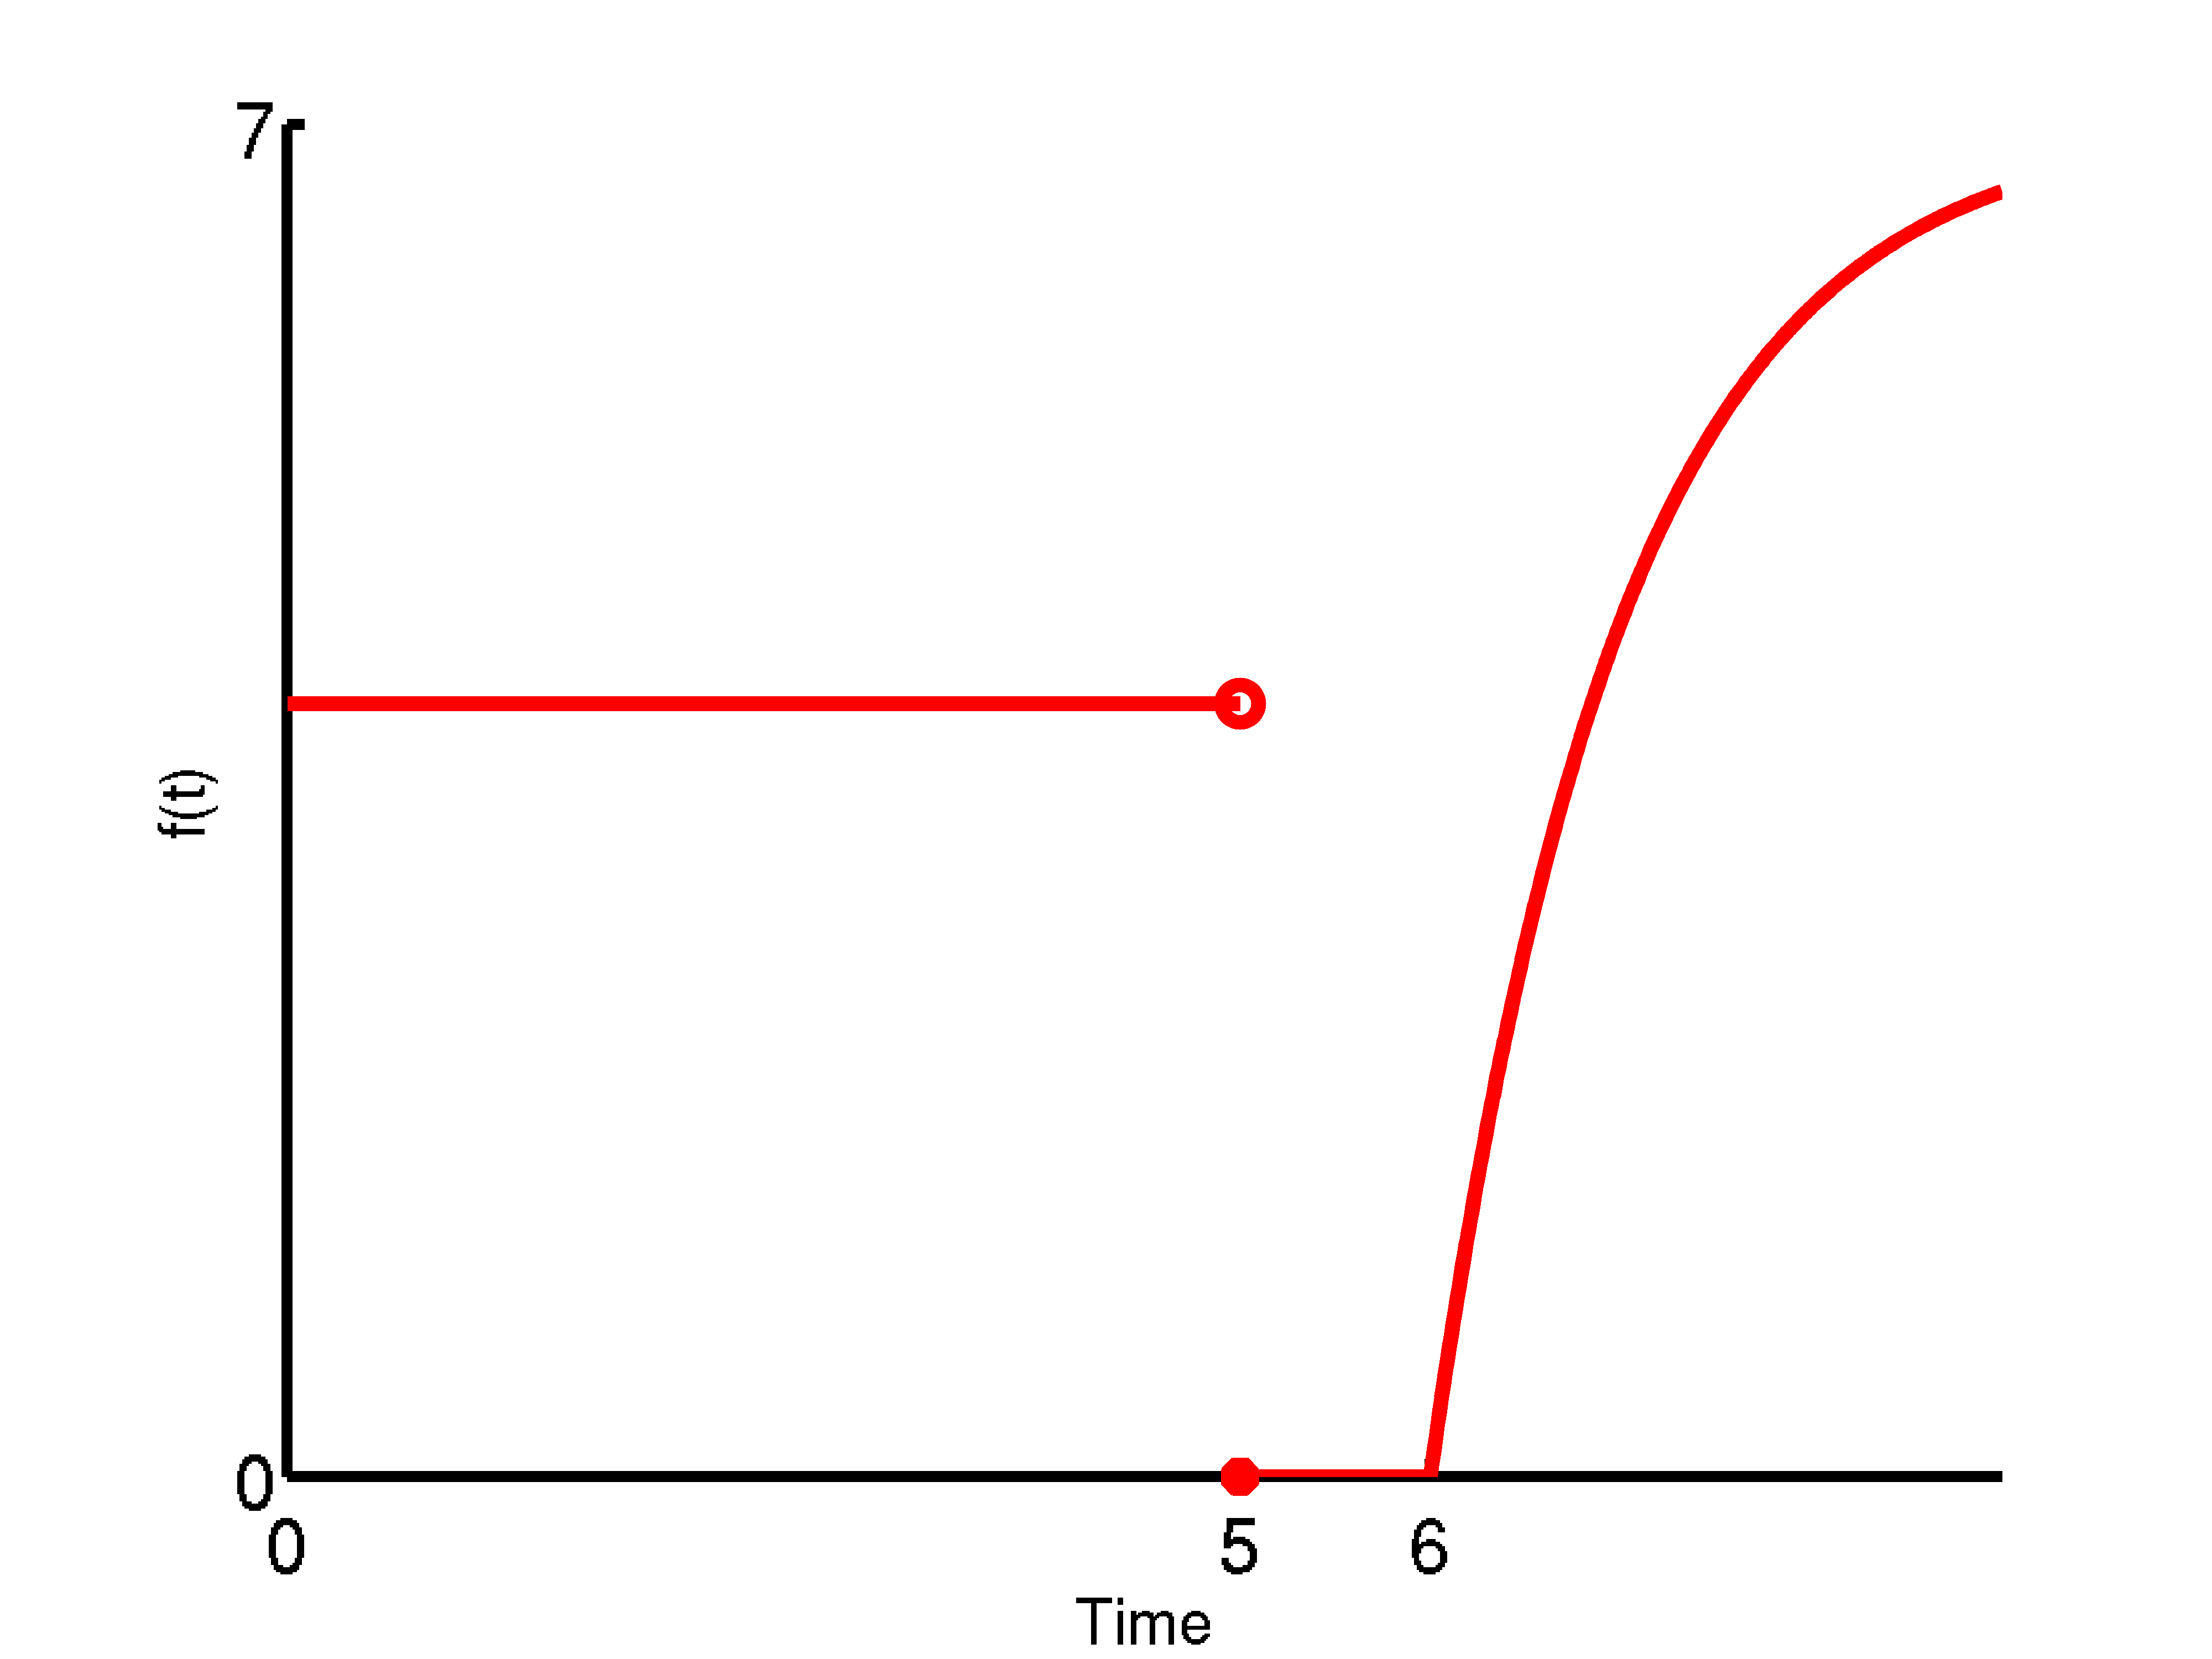
\includegraphics[width=5cm]{img/stepEx6}}

  \begin{eqnarray*}
      f(t) & = & 
      \left\{
        \begin{array}{r@{\hspace{2em}}rcccl}
          7-7e^{-(t-6)} & t & \geq & 6 \\
          0 & 5 & < & t & < & 6 \\
          4 & t & \leq 5 
        \end{array}
      \right.
  \end{eqnarray*}

  \uncover<2->
  {
    \begin{eqnarray*}
      f(t) & = & 4 - 4\cdot\mathrm{step}(t-5) + \lp 7-7e^{-(t-6)}\rp\cdot\mathrm{step}(t-6).
    \end{eqnarray*}
  }


\end{frame}


\subsection{The Laplace Transform of the Unit Step Function}

\begin{frame}
  \frametitle{The Laplace Transform of the Unit Step Function}

  \begin{eqnarray*}
    \laplace{f(t-a)\mathrm{step(t-a)}} & = & 
           \int^\infty_0 f(t-a)\mathrm{step(t-a)} ~ e^{-st} ~ dt, \\
    & = &  \int^\infty_a f(t-a) e^{-st} ~ dt, \\
    & = & \int^\infty_a f(t-a) e^{-s(t-a+a)} ~ dt, \\
    & = & \int^\infty_a f(t-a) e^{-s(t-a)}e^{-as} ~ dt, \\
    & = & e^{-as} \int^\infty_a f(t-a) e^{-s(t-a)} ~ dt, \\
    & = & e^{-as} \int^\infty_0 f(u) e^{-su} ~ du, \\
    & = & e^{-as} \laplace{f} \\
  \end{eqnarray*}

\end{frame}


\begin{frame}
  \frametitle{Example}

  \begin{eqnarray*}
    \laplace{(t-4)^6\cdot\mathrm{step}(t-4)} & = & e^{-4s}\frac{6!}{s^7}.
  \end{eqnarray*}


\end{frame}


\begin{frame}
  \frametitle{Example}

  \begin{eqnarray*}
    \laplace{\cos\lp 4(t-\pi)\rp\cdot\mathrm{step}(t-\pi)} & = & 
    e^{-\pi s}\laplace{\cos(4t)}, \\
    & = & e^{-\pi s} \frac{s}{s^2+16}.
  \end{eqnarray*}

\end{frame}



\begin{frame}
  \frametitle{Example}

  \begin{eqnarray*}
    \laplace{f} & = & e^{-2s}\frac{1}{(s-4)^2}, \\
    \Rightarrow f & = & e^{4(t-2)}(t-2) \cdot \mathrm{step}(t-2).
  \end{eqnarray*}

\end{frame}





\begin{frame}
  \frametitle{Example}

  \begin{eqnarray*}
    8q' + 4q & = & v(t), \\
    q(0) & = & 0, \\
    v(t) & = & 
    \left\{
      \begin{array}{r@{\hspace{2em}}rcl}
        0 & t & \geq & 6 \\
        2 & t & < & 6
      \end{array}
    \right.
  \end{eqnarray*}

  \uncover<2->
  {
    \begin{eqnarray*}
      8q' + 4q & = & 2 - 2 \cdot \mathrm{step}(t-6).
    \end{eqnarray*}
        
  }

\end{frame}


\begin{frame}
  \frametitle{Take the Laplace Transform}

  \begin{eqnarray*}
    8\lp -q(0) + s \laplace{q} \rp + 4 \laplace{q} & = & \frac{2}{s} -
    \frac{2}{s} e^{-6s}.
  \end{eqnarray*}

  \uncover<2->
  {
    \begin{eqnarray*}
      \laplace{q} & = & \frac{1/2}{s(2s+1)} - \frac{1/2}{s(2s+1)} e^{-6s}, \\
      & = & \half \frac{1}{s} - \half \frac{1}{s+\half}
      - \half \frac{1}{s} e^{-6s} + \half \frac{1}{s+\half} e^{-6s}.
    \end{eqnarray*}
  }

  \uncover<3->
  {
    \begin{eqnarray*}
      q & = & \half - \half e^{-t/2} - \half\cdot\mathrm{step}(t-6)
      + \half e^{-(t-6)/2}\cdot\mathrm{step}(t-6).
    \end{eqnarray*}
  }


\end{frame}




% LocalWords:  Clarkson pausesection hideothersubsections rcl rr rcccl dt
